\newpage

\begin{figure}[H]
    \centering
    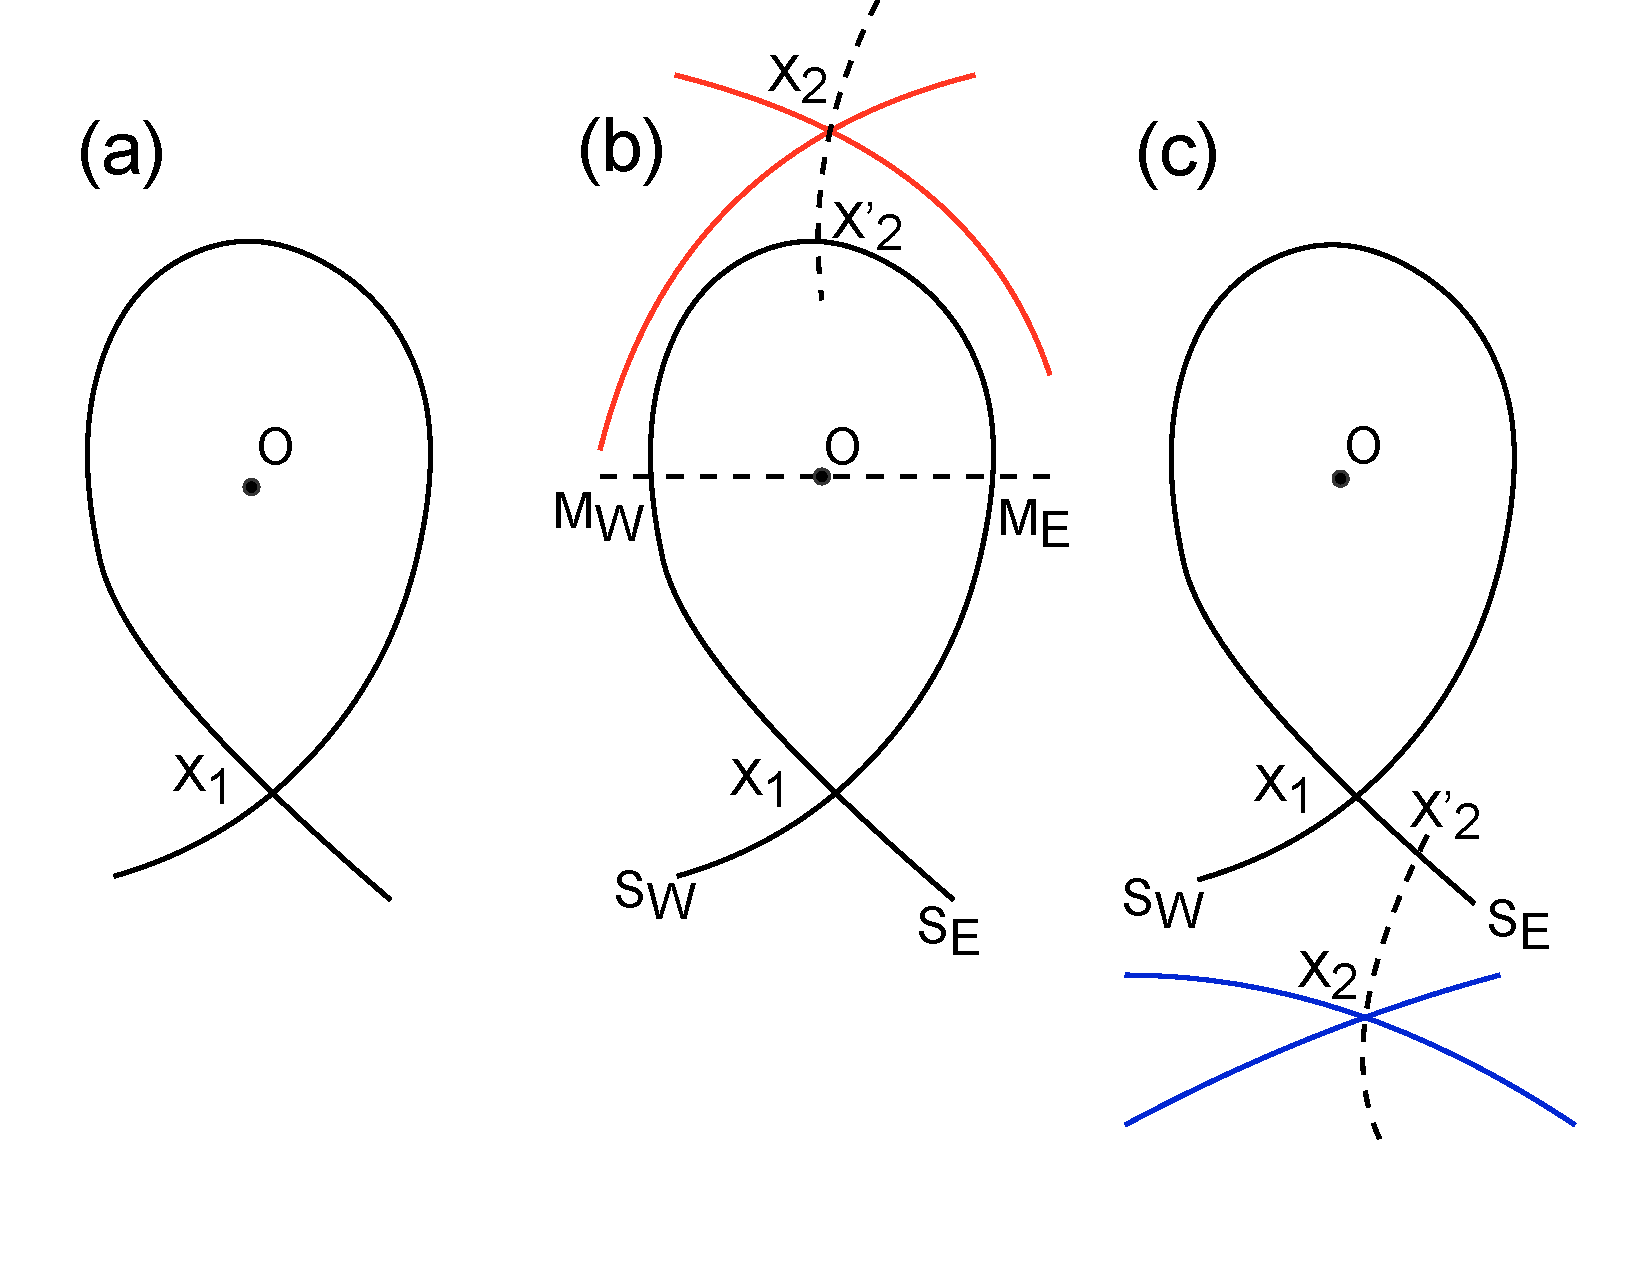
\includegraphics[width=\linewidth]{figures/all_conf.pdf}

    \caption{Topological possibilites with one and two X-points. As
    explained in the main text, case (a) is a single-null
    configuration; case (b) with the secondary X-point in the
    common-flux region has five variations, depending on the location
    of the projection point $X_2^{\prime}$; case (c) with the
    secondary X-point in the private-flux region has two variations
    depending on the location of the projection point $X_2^{\prime}$.
    The East-West notation for the two midplane points and the two
    strike points is based on designating the direction from the
    primary X-point toward the O-point as ``North''. This is invariant
    notation, independent on whether the primary X-point is at the
    top, at the bottom, or anywhere else.}

    \label{fig:all_conf}
\end{figure}

%<<<<<<< Updated upstream
%\begin{figure}[H]
%    \centering
%    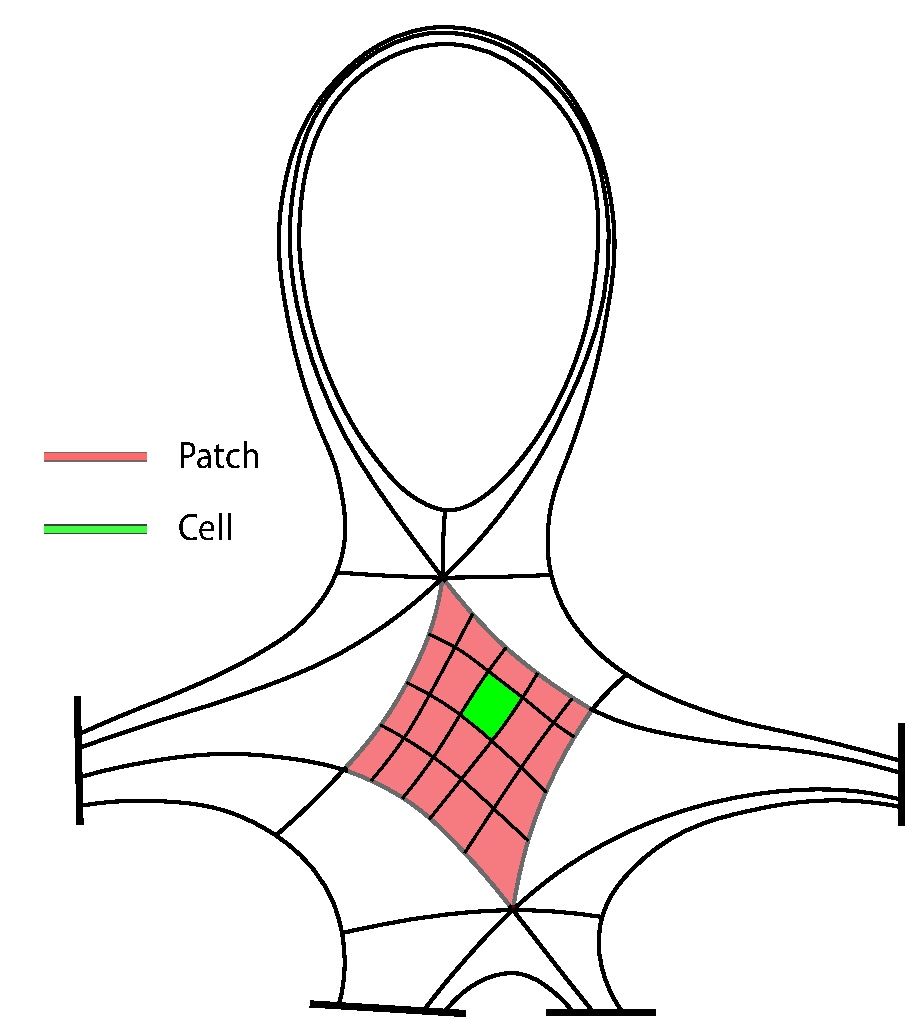
\includegraphics[width=0.5\linewidth]{figures/geometry_render.pdf}  % scale=0.35
%    \caption{\label{fig:geo_collection} INGRID geometric objects are used to represent an arbitrary magne%tic topology. Here we explicitly see a Patch, Cell, and Line. Points are implicitly shown by a Line and C%ell object definition.}
%\end{figure}

% \begin{figure}[H]
%     \centering
%     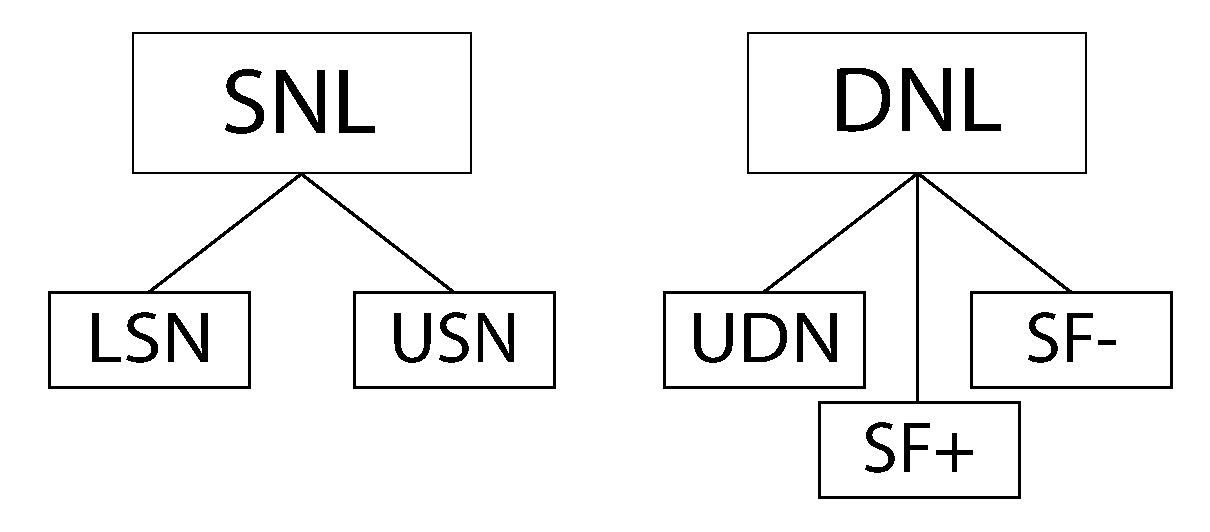
\includegraphics[width=\linewidth]{figures/config_group.pdf}
%     \caption{Categorizing magnetic topologies by number of x-points induces a natural design pattern for a grid generator.}
%     \label{fig:config_group}
% \end{figure}

% \begin{figure}[H]
%     \centering
%     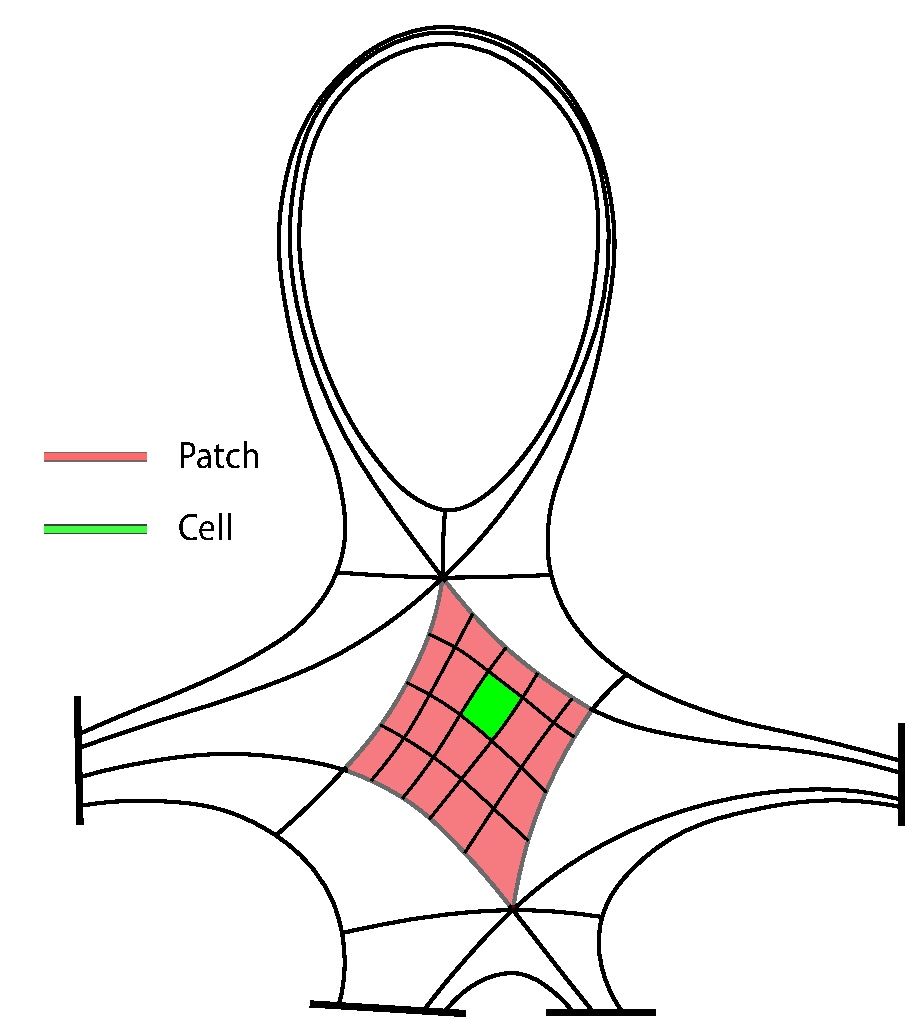
\includegraphics[width=0.35\linewidth]{figures/geometry_render.pdf}  % scale=0.35
%     \caption{\label{fig:geo_collection} INGRID geometric objects are used to represent an arbitrary magnetic topology. Here we explicitly see a Patch, Cell, and Line. Points are implicitly shown by a Line and Cell object definition.}
% \end{figure}

%\begin{figure}[H]
%    \centering
%    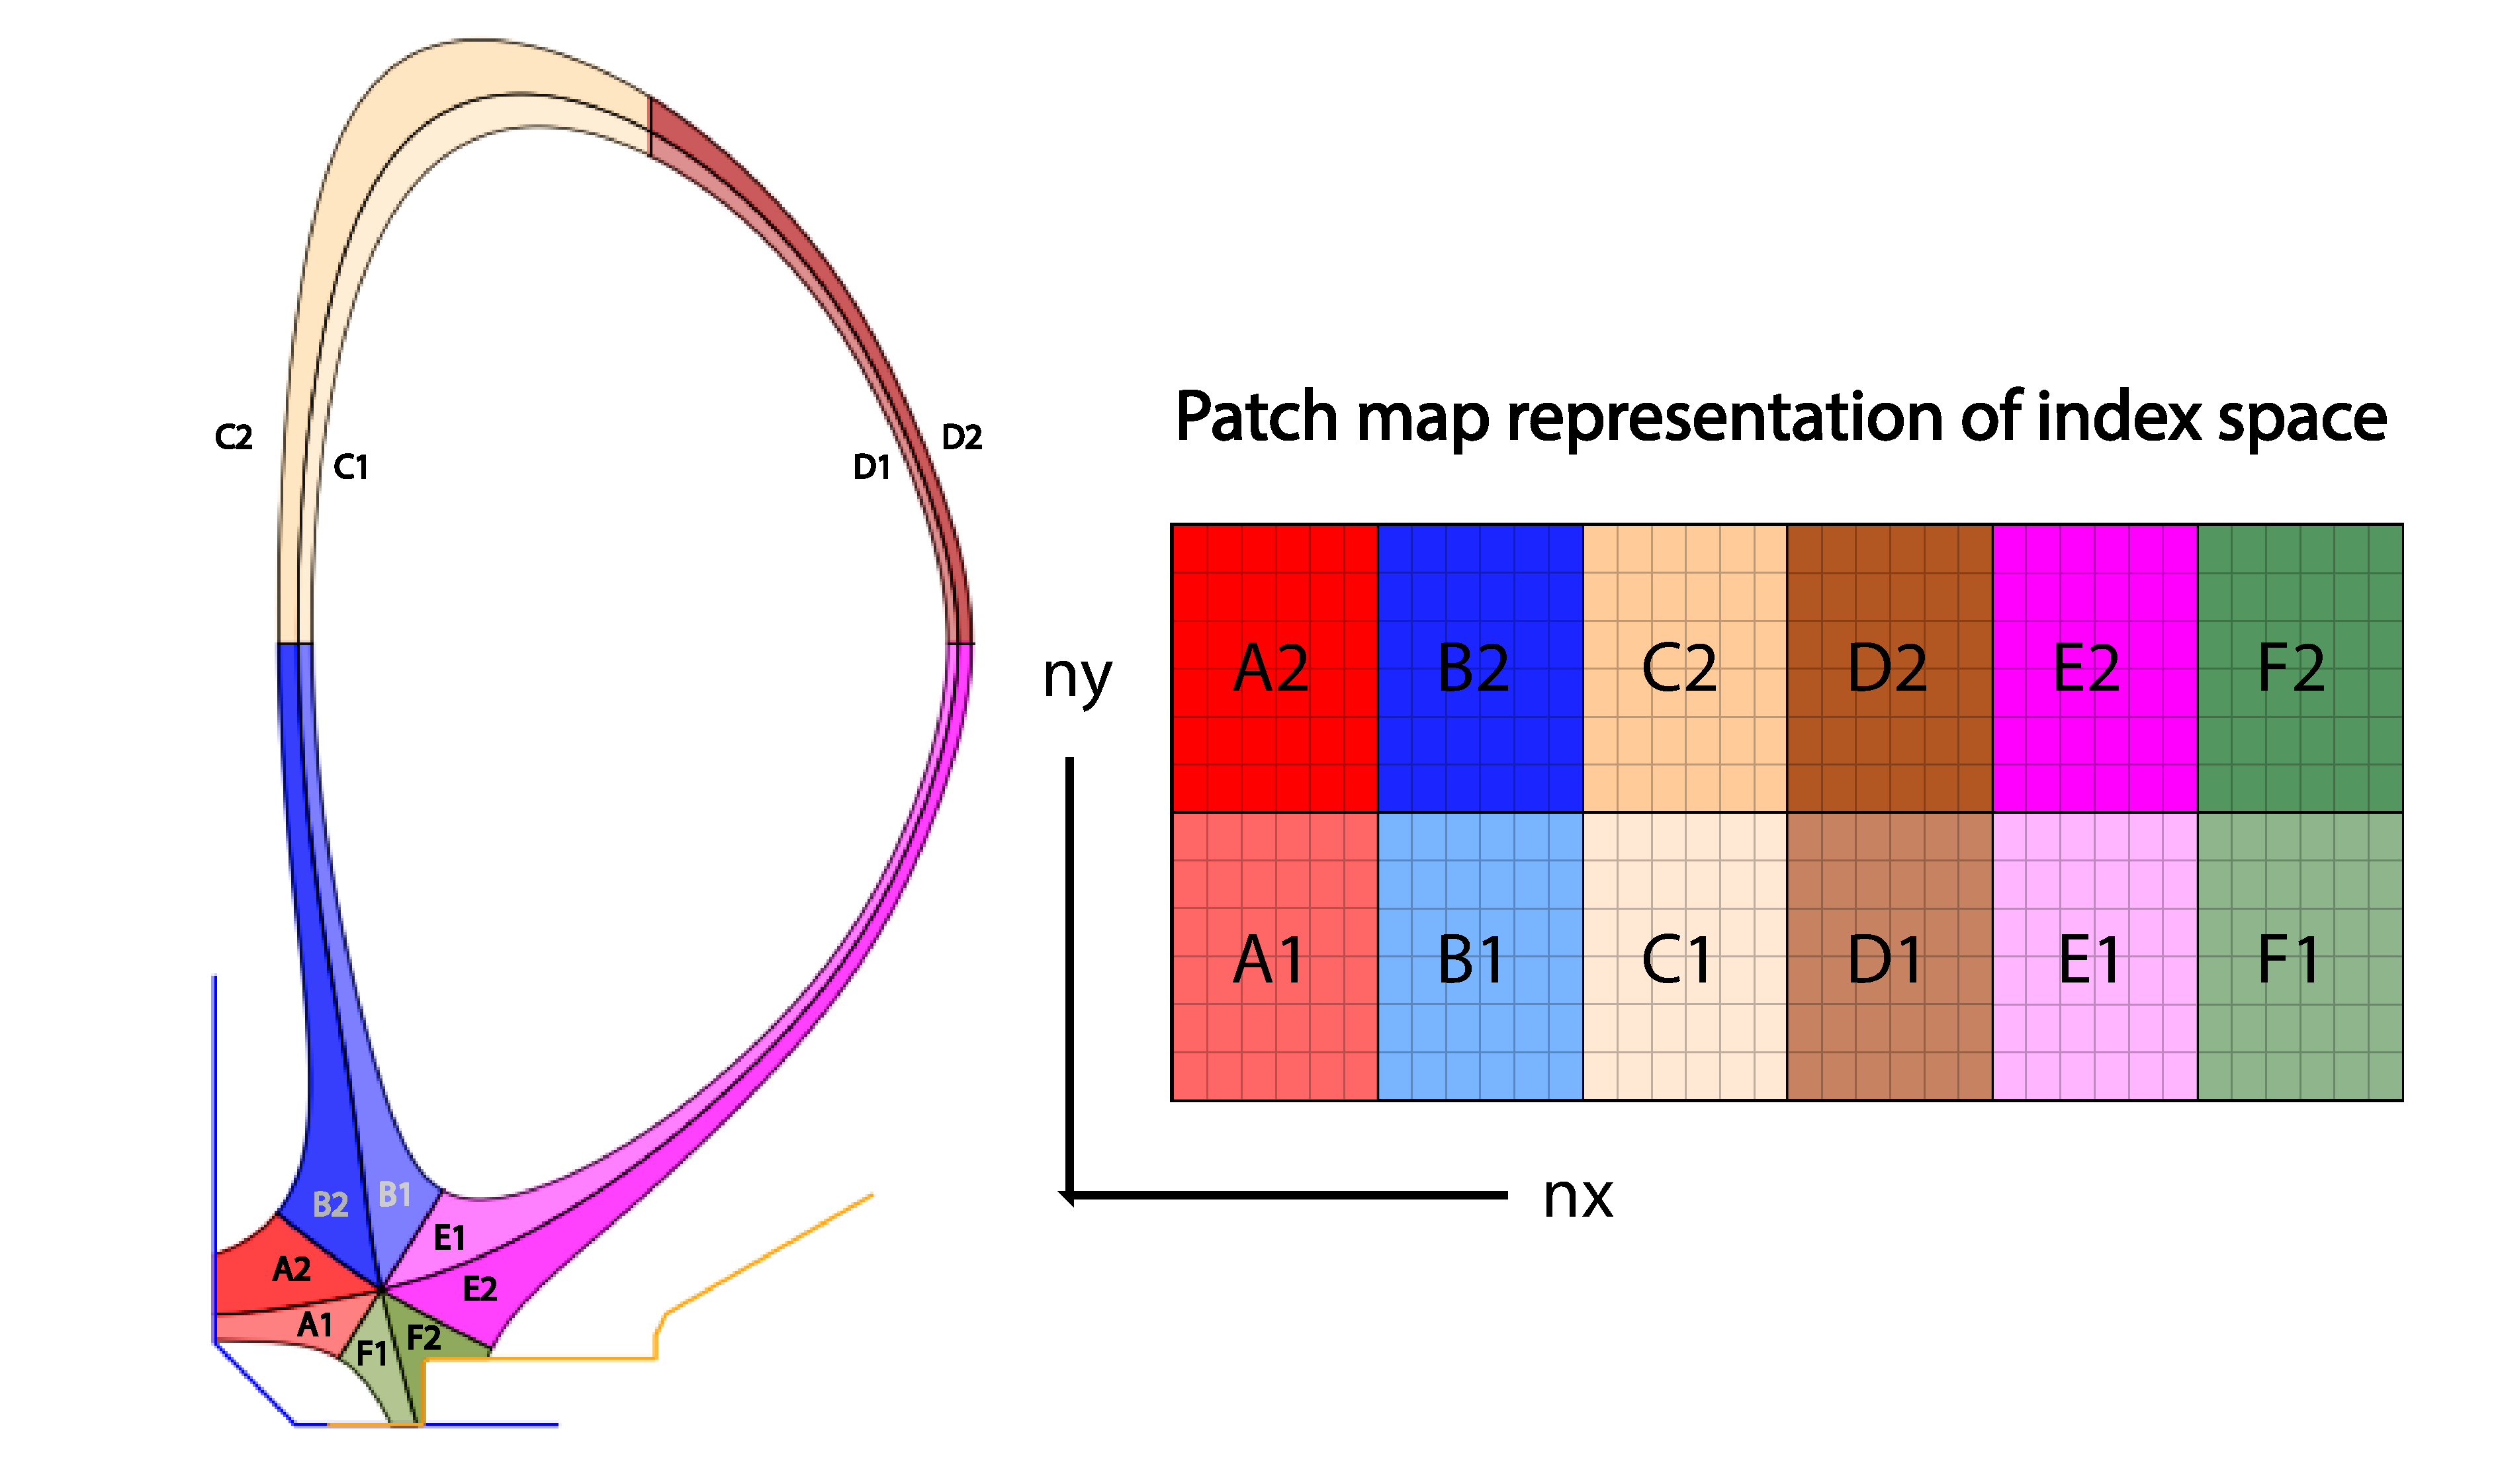
\includegraphics[width=\linewidth]{figures/patch_index_space.pdf}
%    \caption{The Patch-Map of an SNL configuration and it's correspondence to a grid in index space. Indi%vidual Patch objects and their region in index space are labeled with a two-character key.}
%    \label{fig:snl_patch_index_space}
%\end{figure}

%\begin{figure}[H]
%    \centering
%    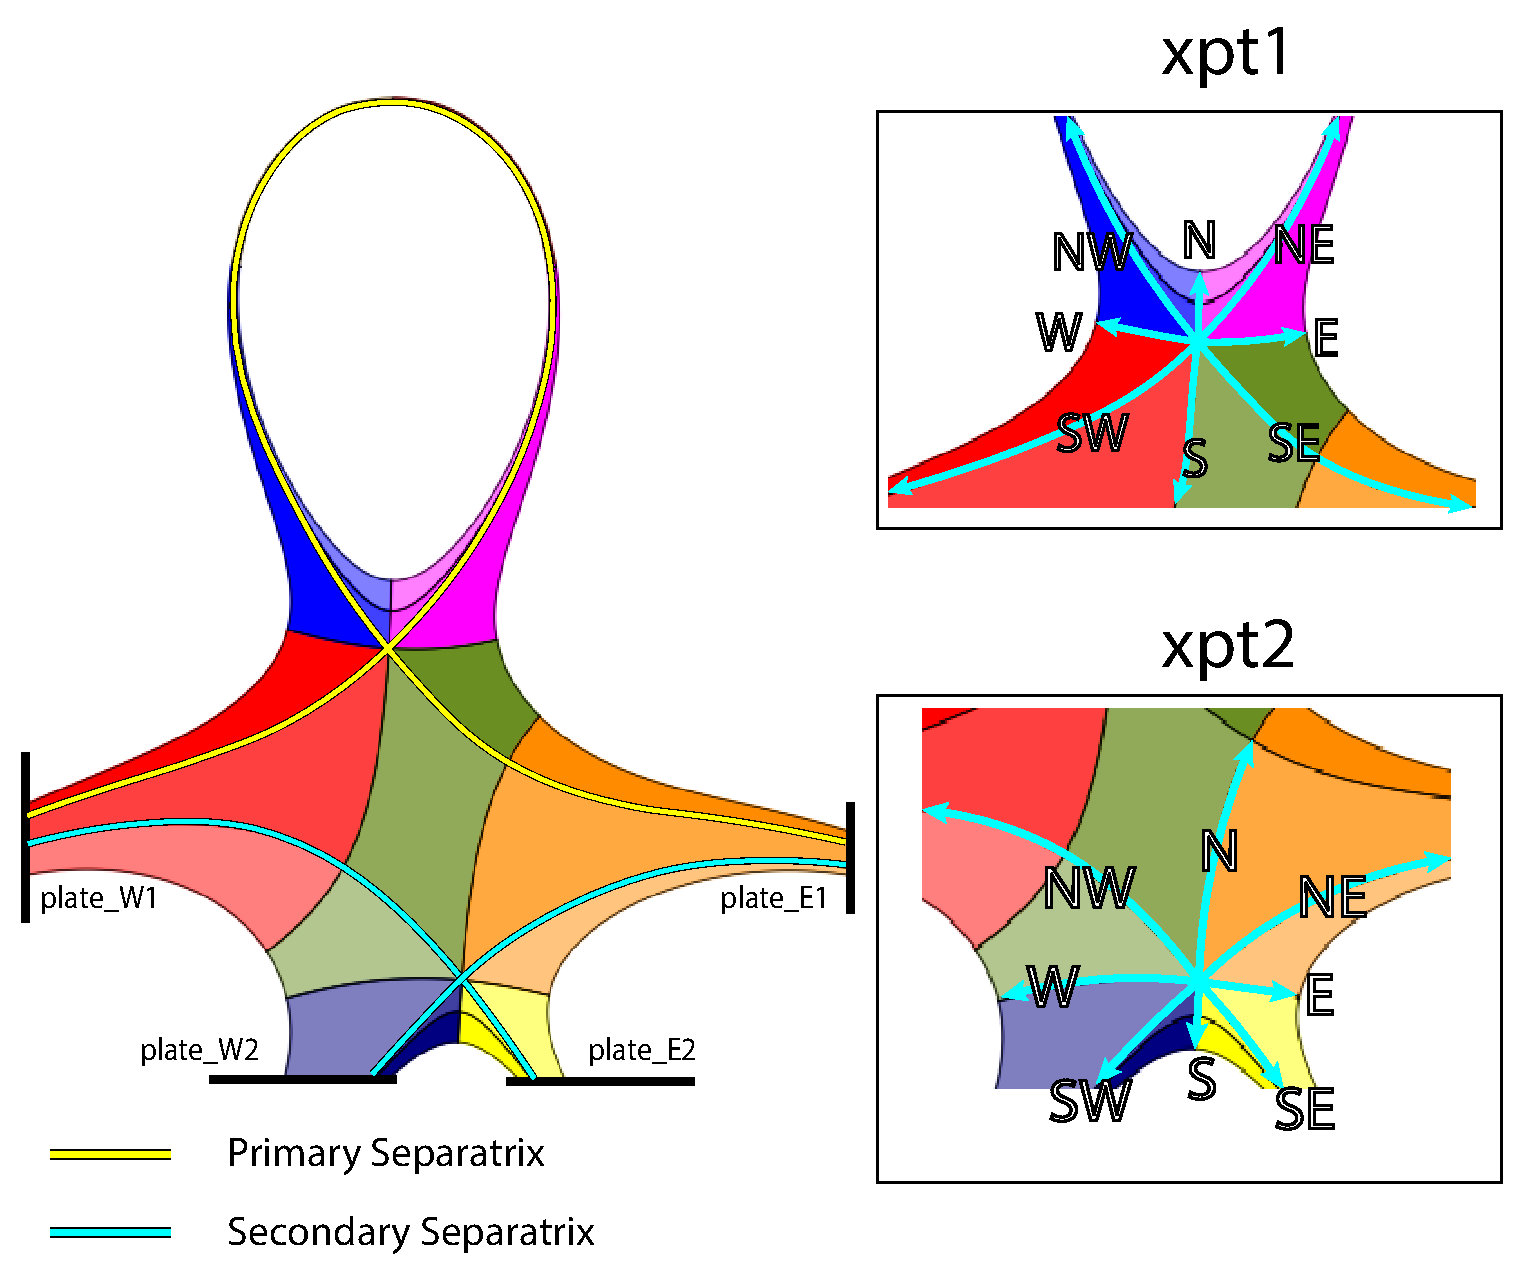
\includegraphics[width=\linewidth]{figures/xpt_2_directions.pdf}
%    \caption{An SF75 divertor configuration illustrating the primary x-point and secondary x-point N-S-E-%W labeling convention.}
%    \label{fig:xpt_2_directions}
%\end{figure}
%=======


%\begin{figure}[H]
%    \centering
%    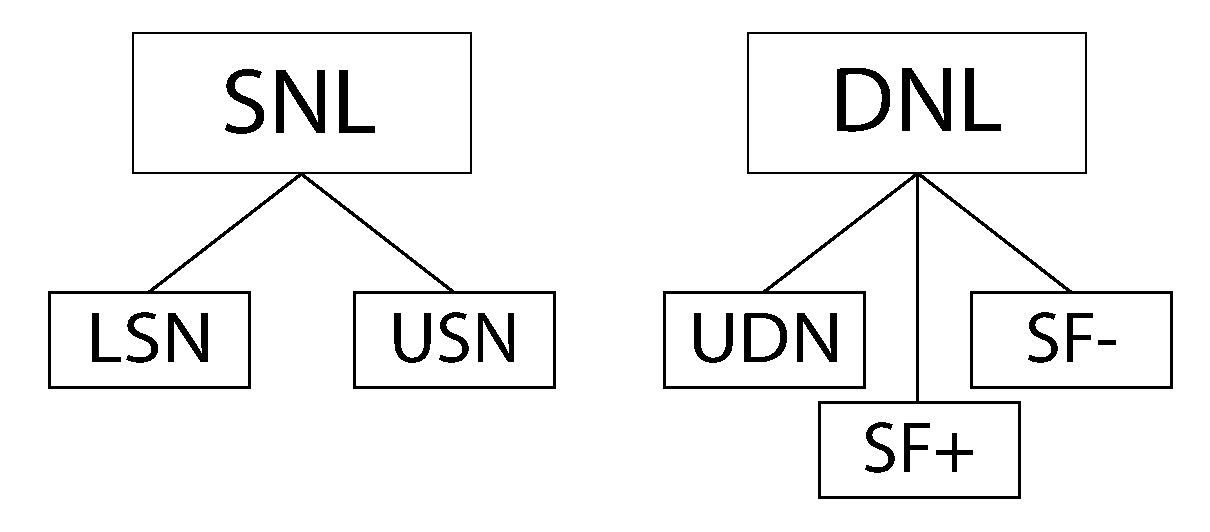
\includegraphics[width=\linewidth]{figures/config_group.pdf}
%    \caption{Categorizing magnetic topologies by number of x-points induces a natural design% pattern for a grid generator.}
%    \label{fig:config_group}
%\end{figure}

\begin{figure}[H]
    \centering
    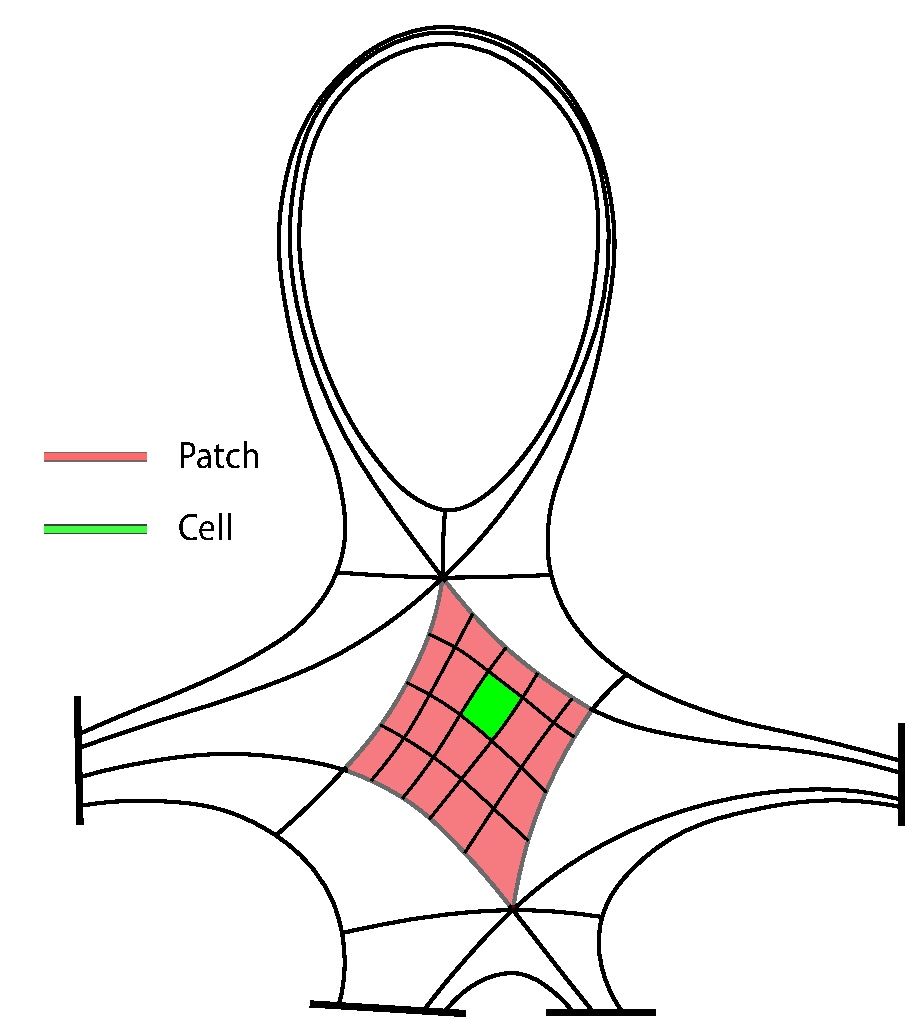
\includegraphics[width=0.5\linewidth]{figures/geometry_render.pdf}  % scale=0.35
    \caption{INGRID Patch-Map; a subgrid is shown on one of the patches}
    \label{fig:patchmap_subgrid}
\end{figure}

%\begin{figure}[H]
%    \centering
%    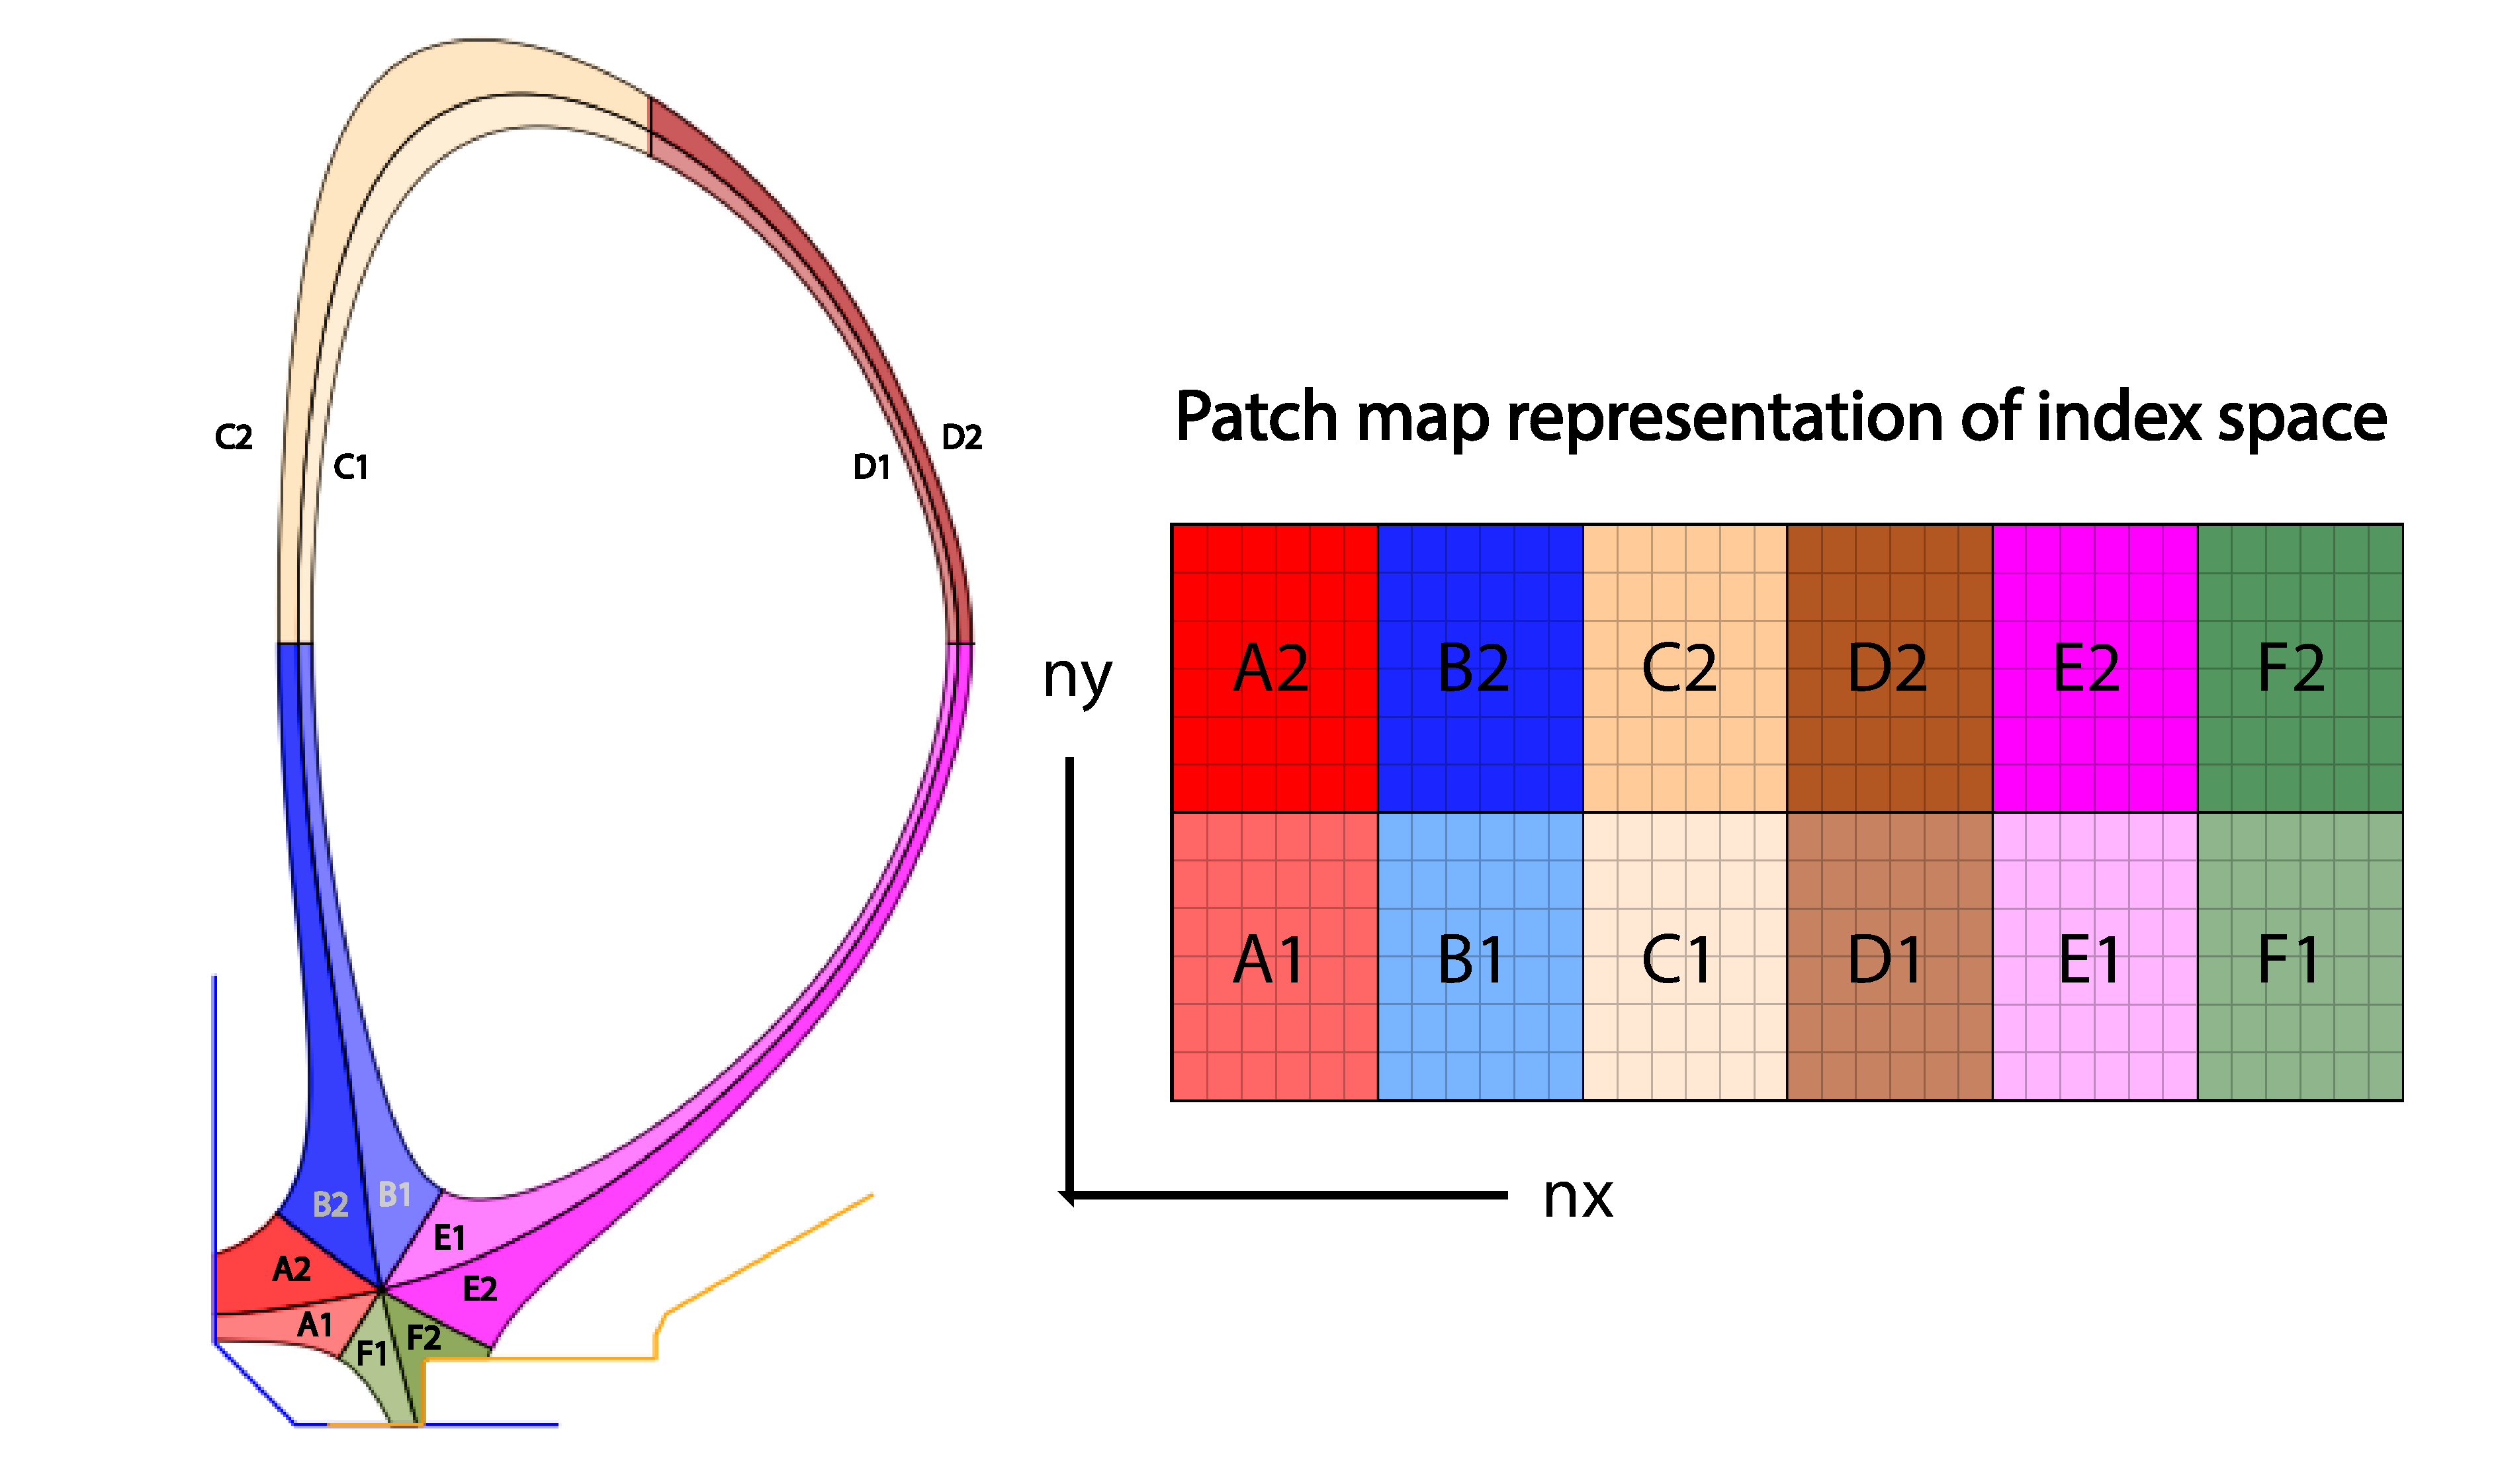
\includegraphics[width=\linewidth]{figures/patch_index_space.pdf}
%    \caption{The Patch-Map of an SNL configuration and it's correspondence to a grid in index space. Individual Patch objects and their region in index space are labeled with a two-character key.}
%    \label{fig:snl_patch_index_space}
%\end{figure}

%\begin{figure}[H]
%    \centering
%    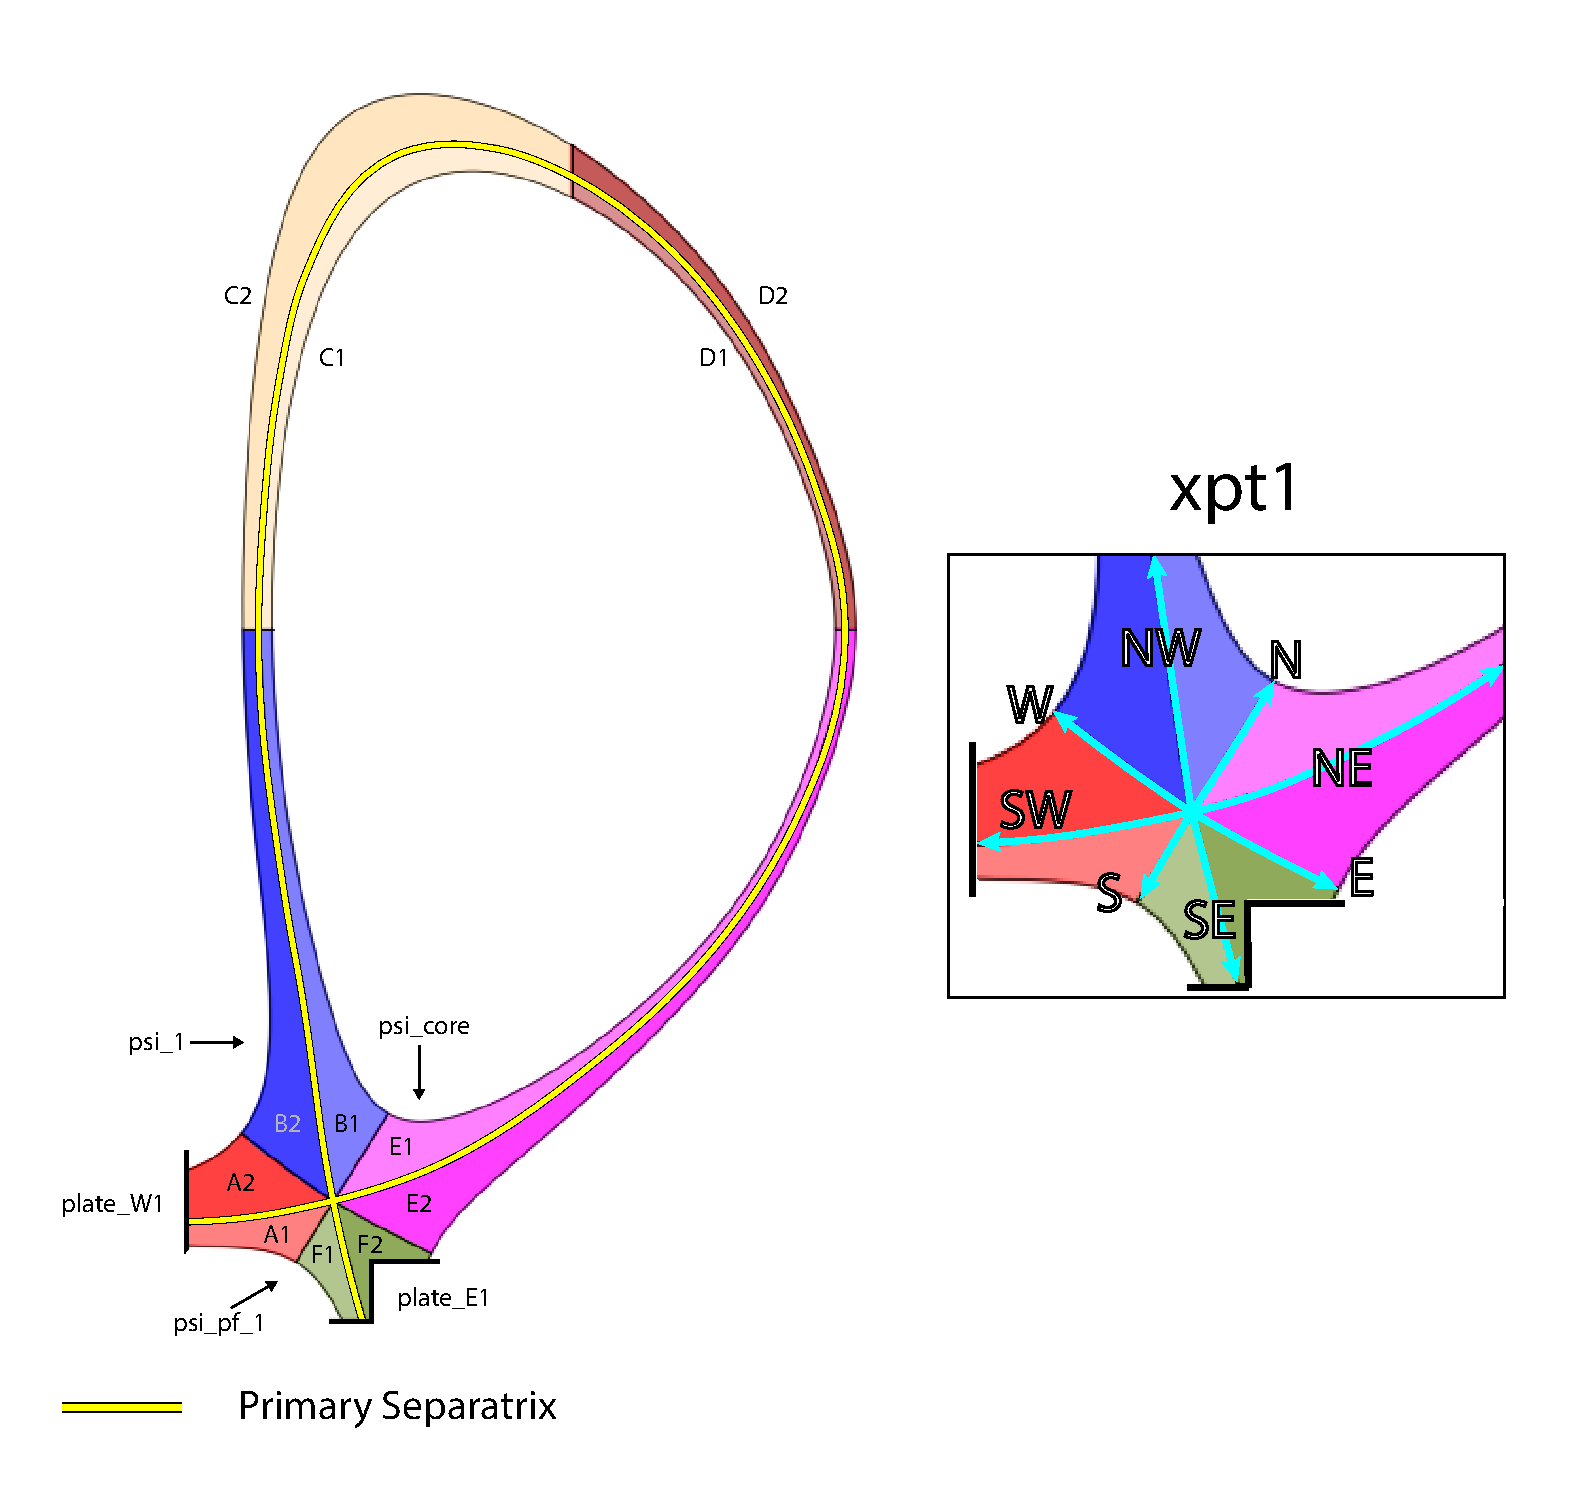
\includegraphics[width=\linewidth]{figures/xpt_1_directions.pdf}
%    \caption{An SNL divertor configuration illustrating the primary x-point's N-S-E-W labeling convention.}
%    \label{fig:xpt_1_directions}
%\end{figure}

%\begin{figure}[H]
%    \centering
%    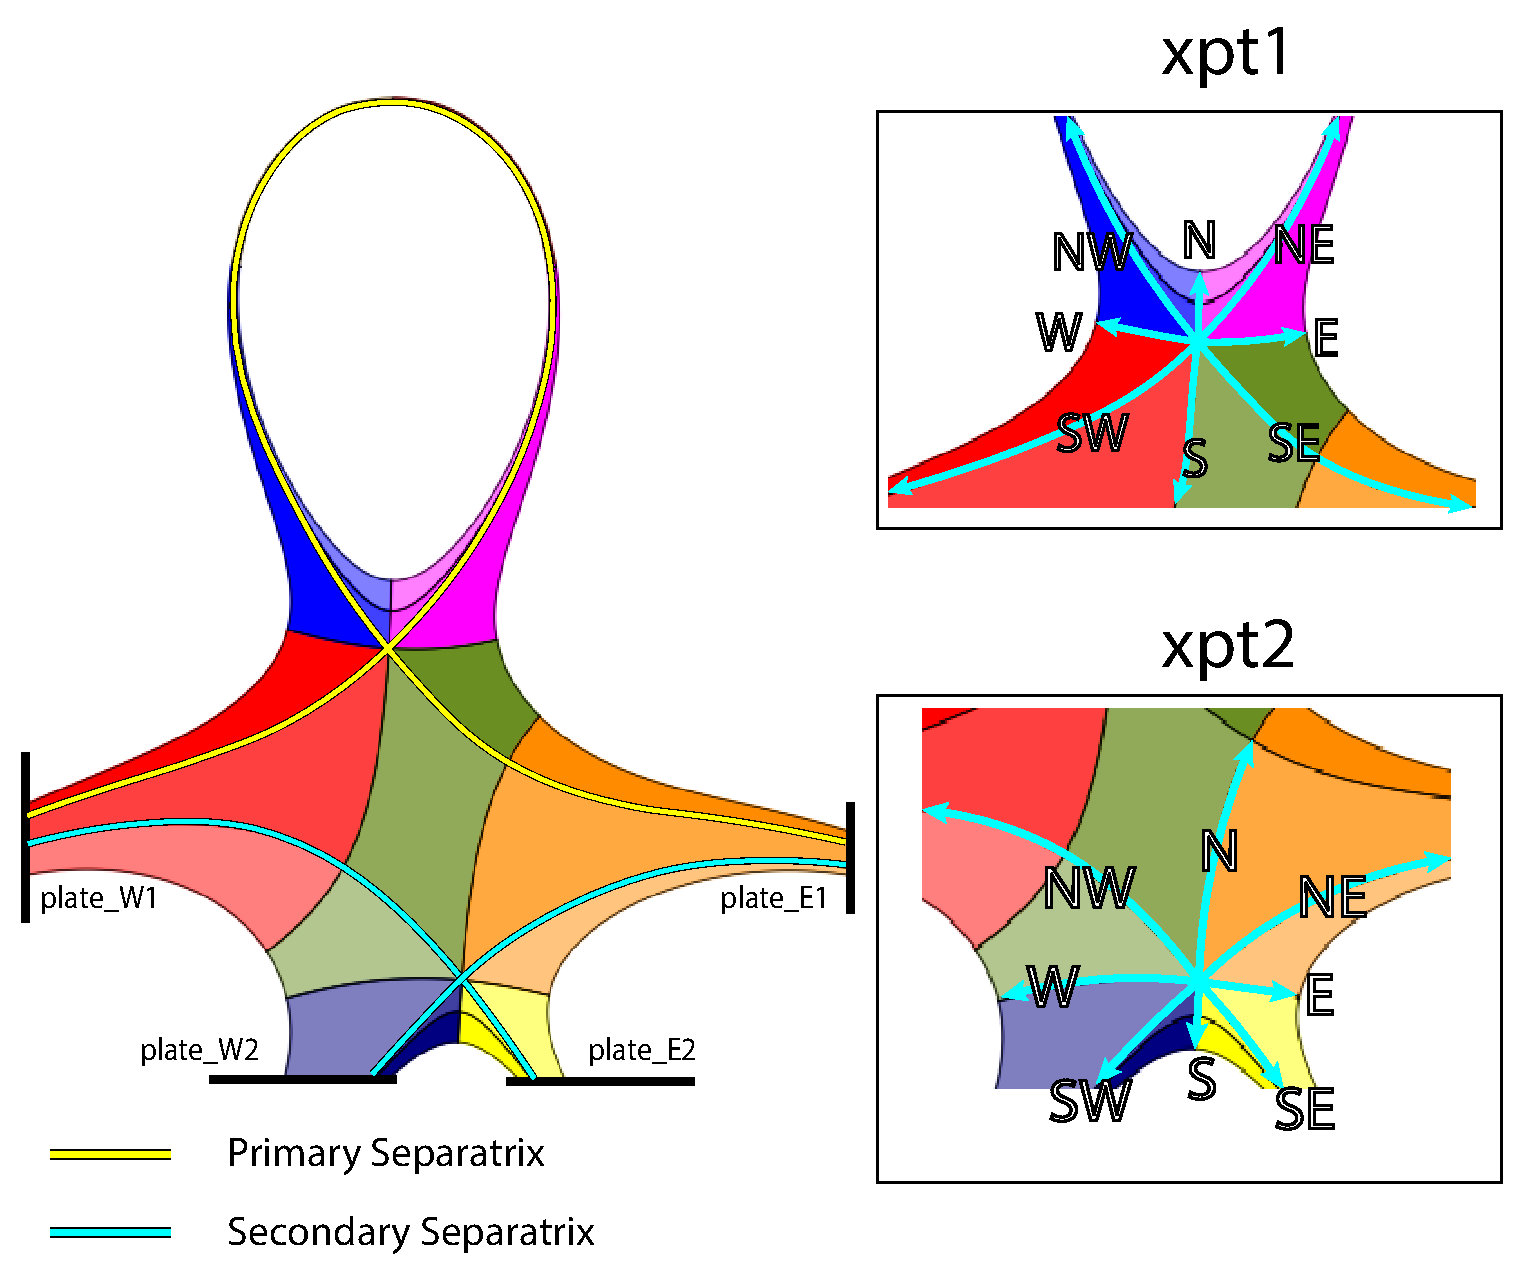
\includegraphics[width=\linewidth]{figures/xpt_2_directions.pdf}
%    \caption{An SF75 divertor configuration illustrating the primary x-point and secondary x-point N-S-E-W labeling convention.}
%    \label{fig:xpt_2_directions}
%\end{figure}
%>>>>>>> Stashed changes

% \begin{figure}[H]
%     \centering
%     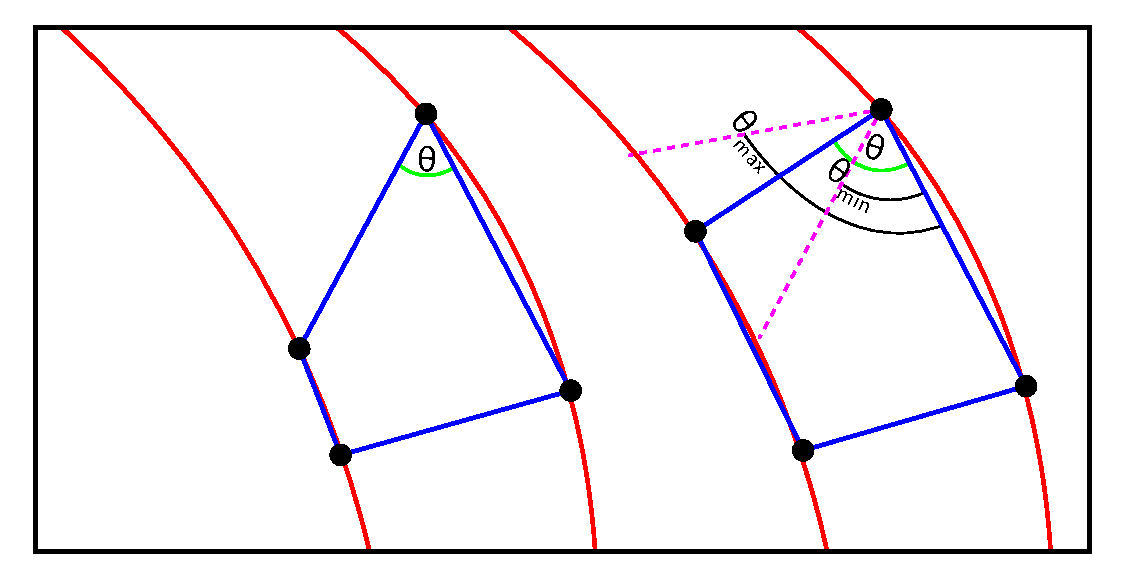
\includegraphics[width=\linewidth]{figures/cell_shearing_diagram.pdf}
%     \caption{Schematic of distortion\_correction applied to a Cell. Before distortion\_correction is applied (left), Cell shearing may be extreme. Enforcing an angle threshold with distortion\_correction (right) makes the grid close to locally orthogonal.}
%     \label{fig:cell_shearing}
% \end{figure}

\begin{figure}[H]
    \centering
    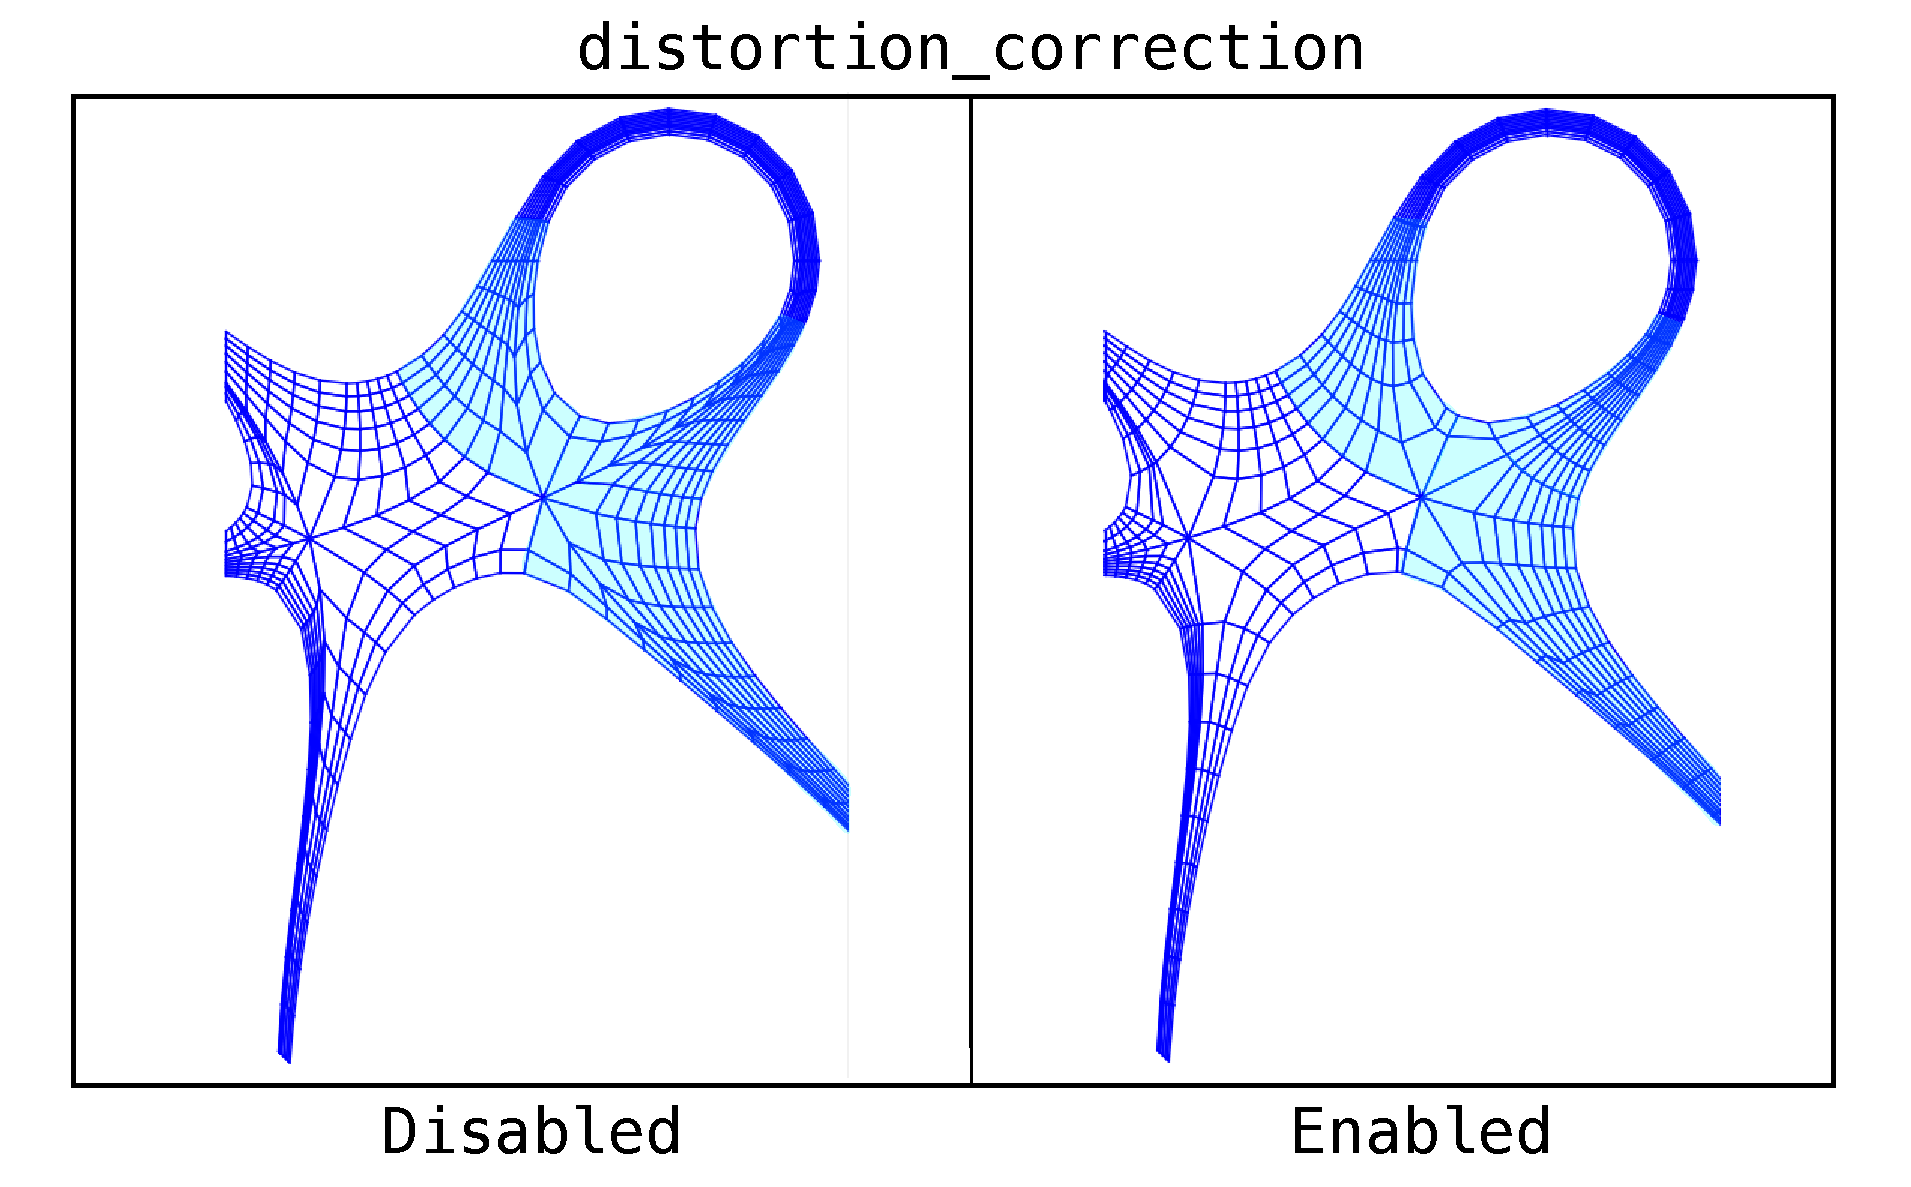
\includegraphics[width=\linewidth]{figures/distortion_correction_1.pdf}
    \caption{Comparison of SF135 grids generated with and without activation of the distortion\_correction tool. Highlighted regions illustrate regions of notably improved grid orthogonality.}
    \label{fig:distortion_correction}
\end{figure}

\begin{figure}[H]
    \centering
    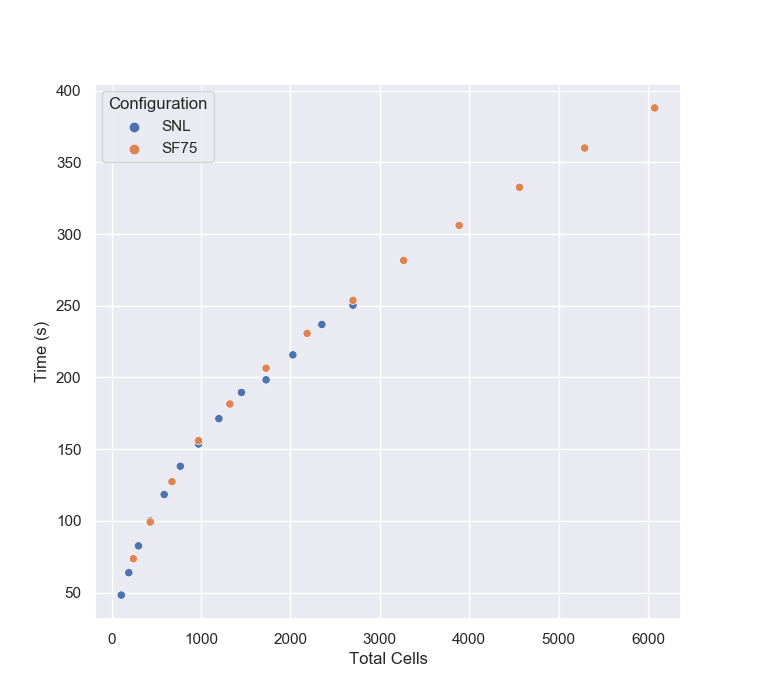
\includegraphics[width=\linewidth]{figures/benchmark/benchmark_grid_scaling.png}
    \caption{Scaling of grid generation follows a sublinear trend independent of configuration. Grids were generated with $n\times n$ many cells per Patch with $n = \{3, 4, 5, \dots, 15\}$. With $n \times n$ subgrid dimensions, SNL configurations contain $12n^2$ many cells, whereas SF75 configurations contain $27n^2$ many cells.}
    \label{fig:benchmark_grid_scaling}
\end{figure}

\begin{figure}[H]
    \centering
        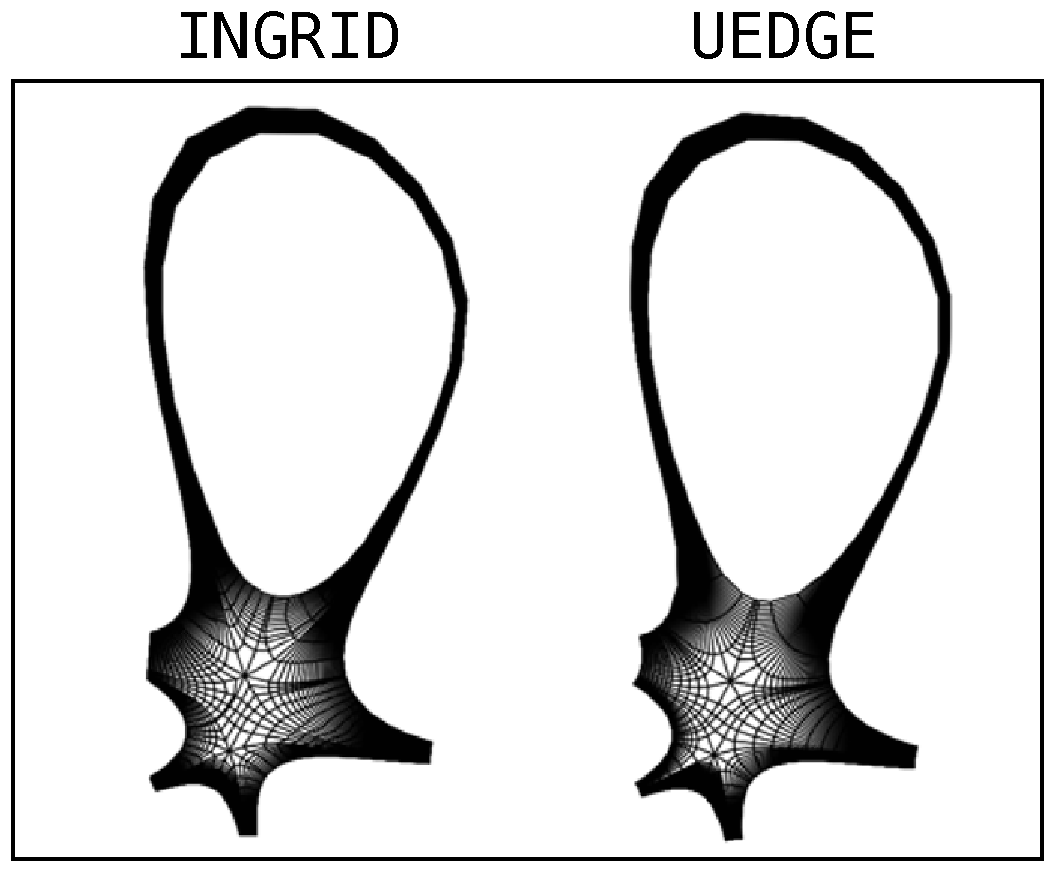
\includegraphics[width=0.9\textwidth]{figures/benchmark/gridue_both.pdf}
        \caption{INGRID and UEDGE generated grids used for the benchmark calculations.}
        \label{fig:ingrid_grid}
\end{figure}
\begin{figure}[H]
    \centering
        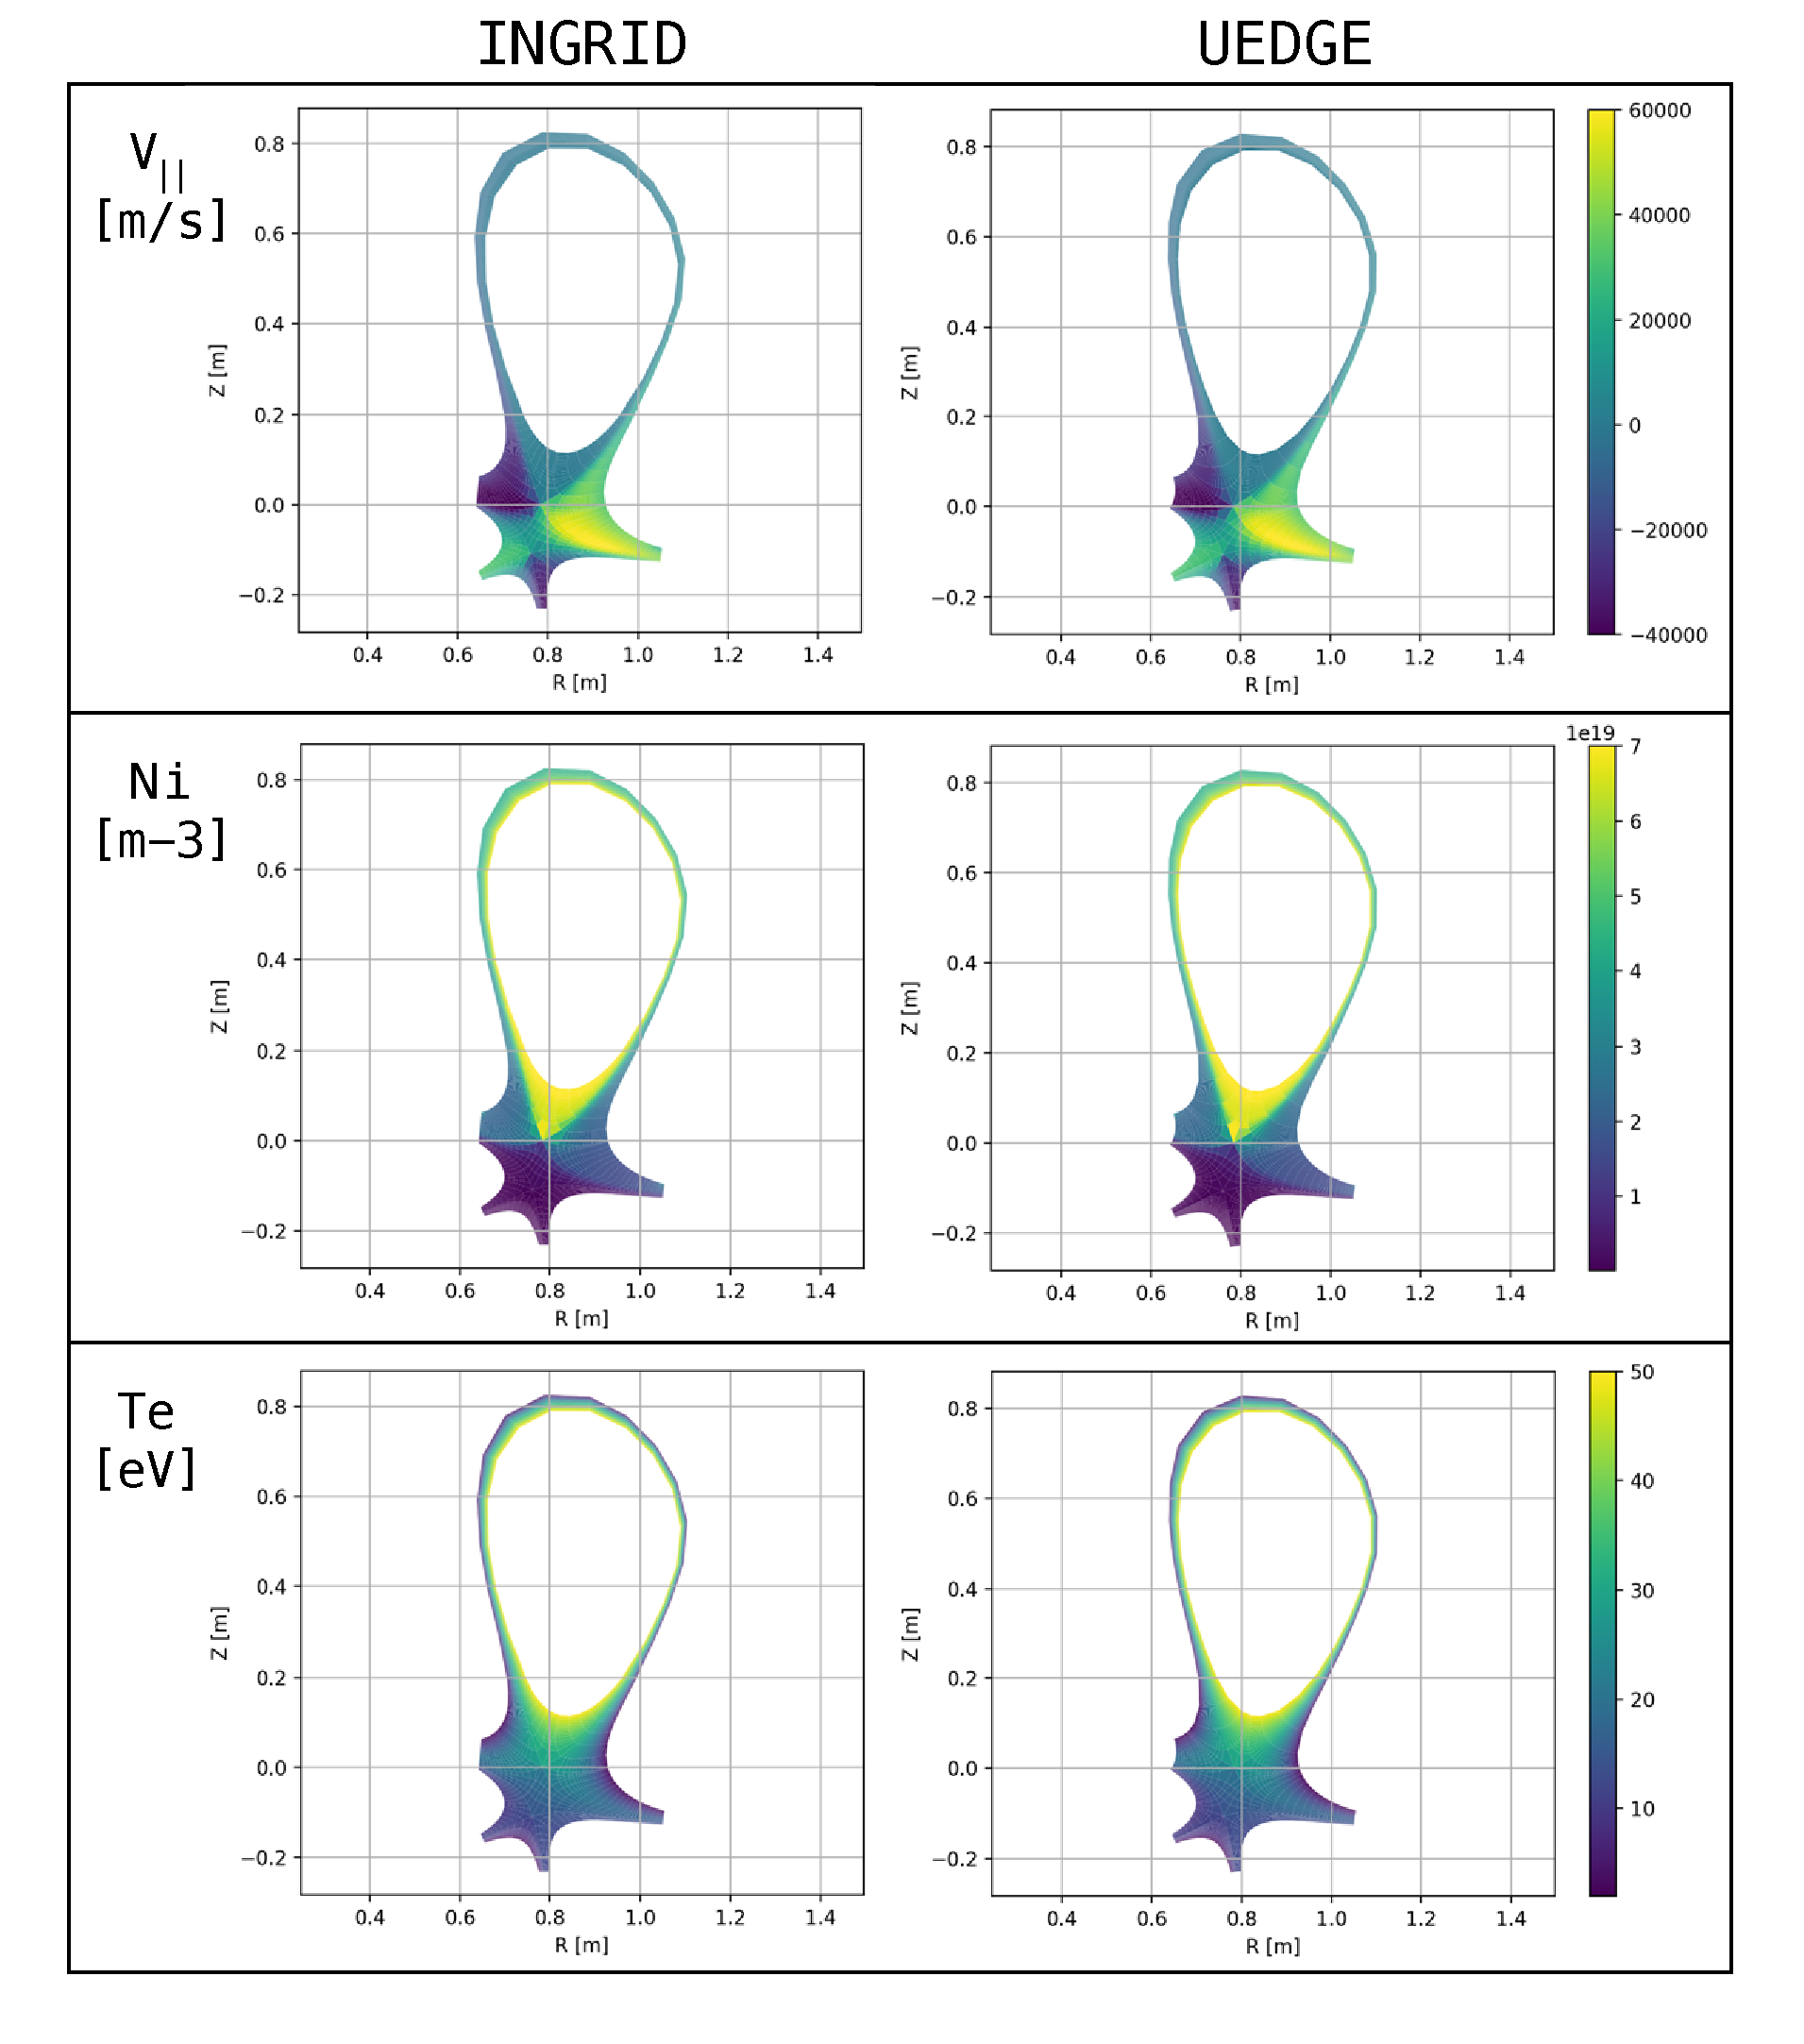
\includegraphics[width=\textwidth]{figures/benchmark/BenchmarkCollection.pdf}
        \caption{Results of the benchmark calculations run on INGRID and UEDGE generated grids.}
        \label{fig:benchmark_collection}
\end{figure}

%%%\section{Supported divertor configurations}
\begin{figure}[H]
    \centering
        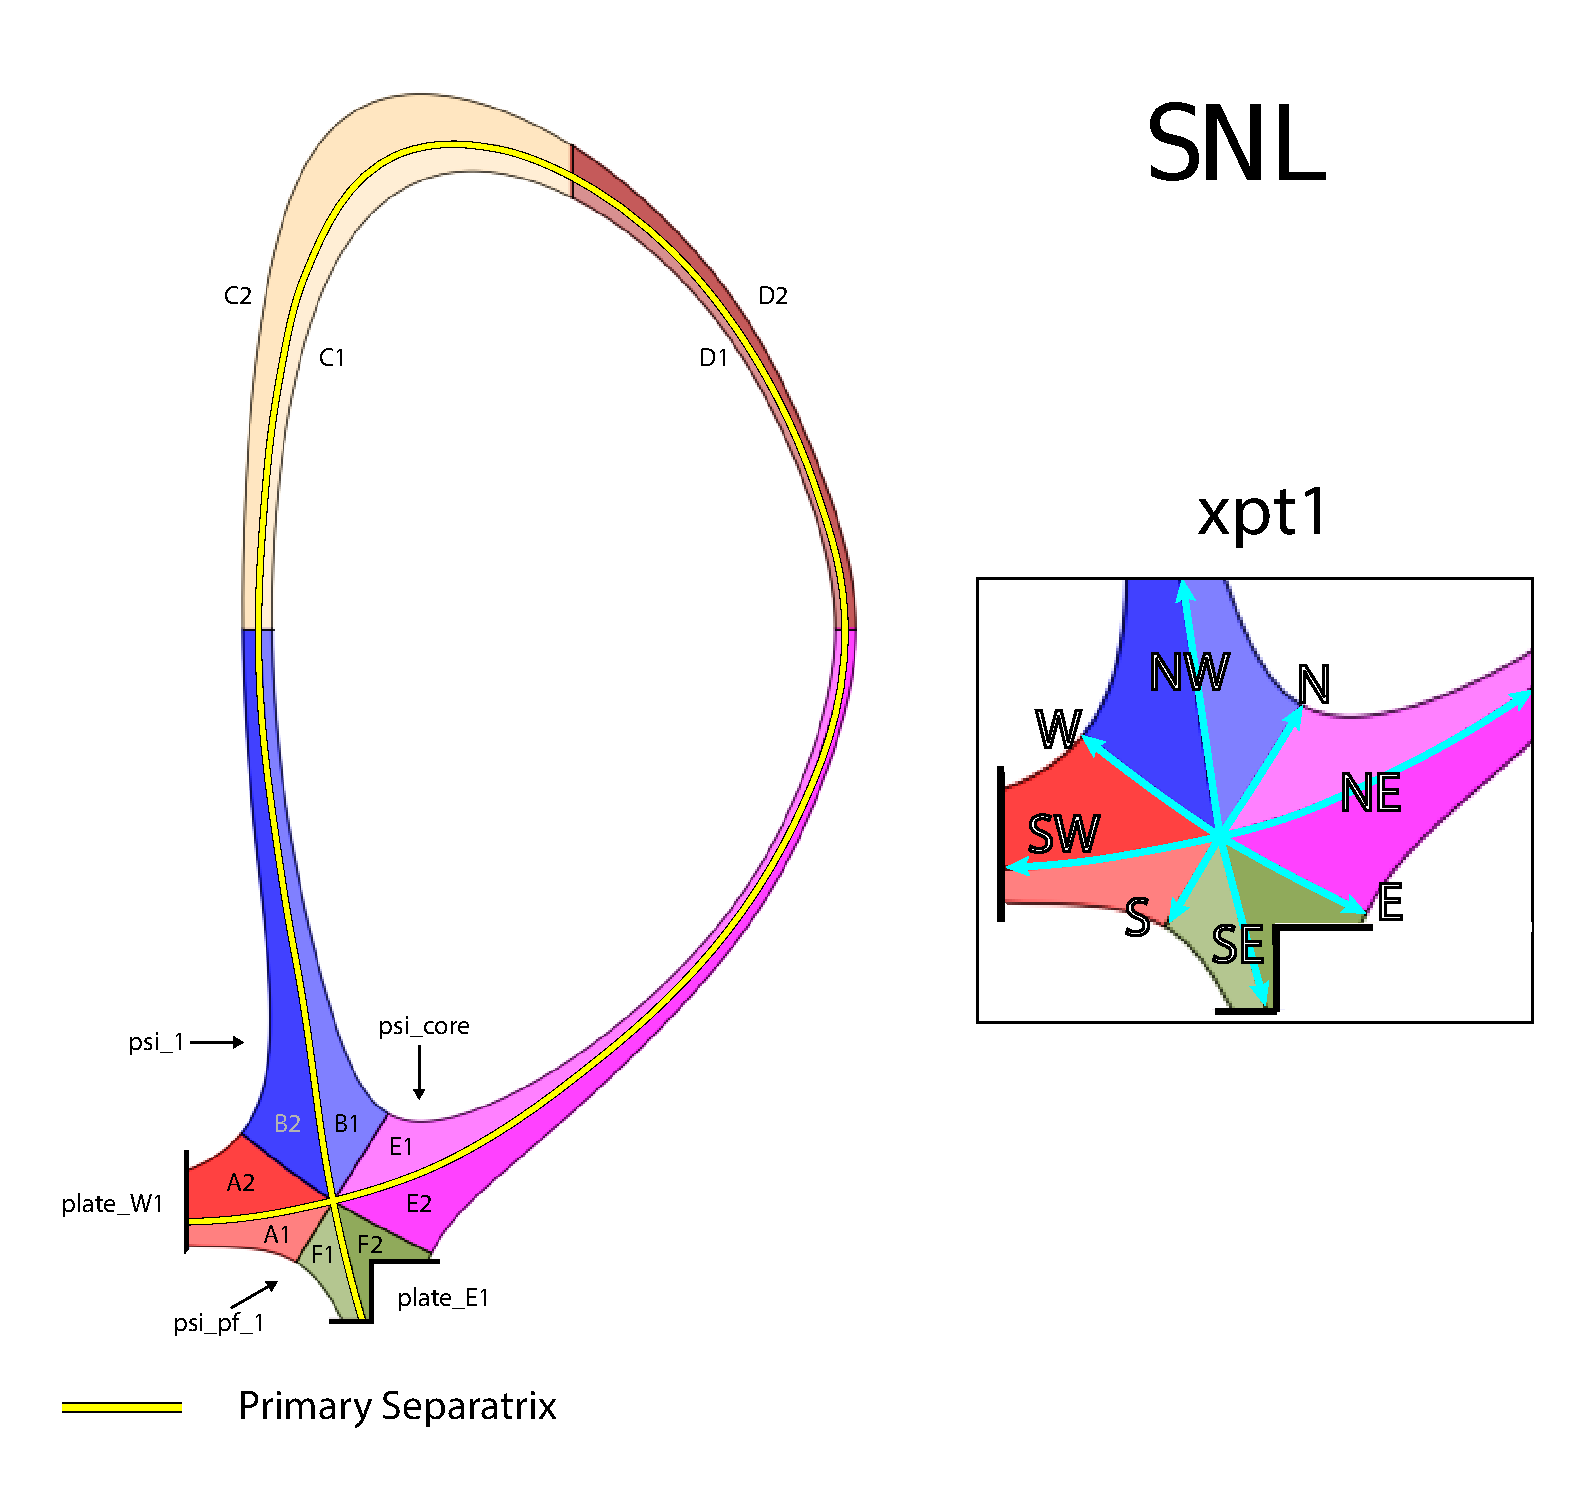
\includegraphics[width=\textwidth]{figures/configurations/SNL_collection.pdf}
        \caption{SNL Patch-Map}
        \label{fig:snl_patch_map}
\end{figure}

\begin{figure}[H]
    \centering
        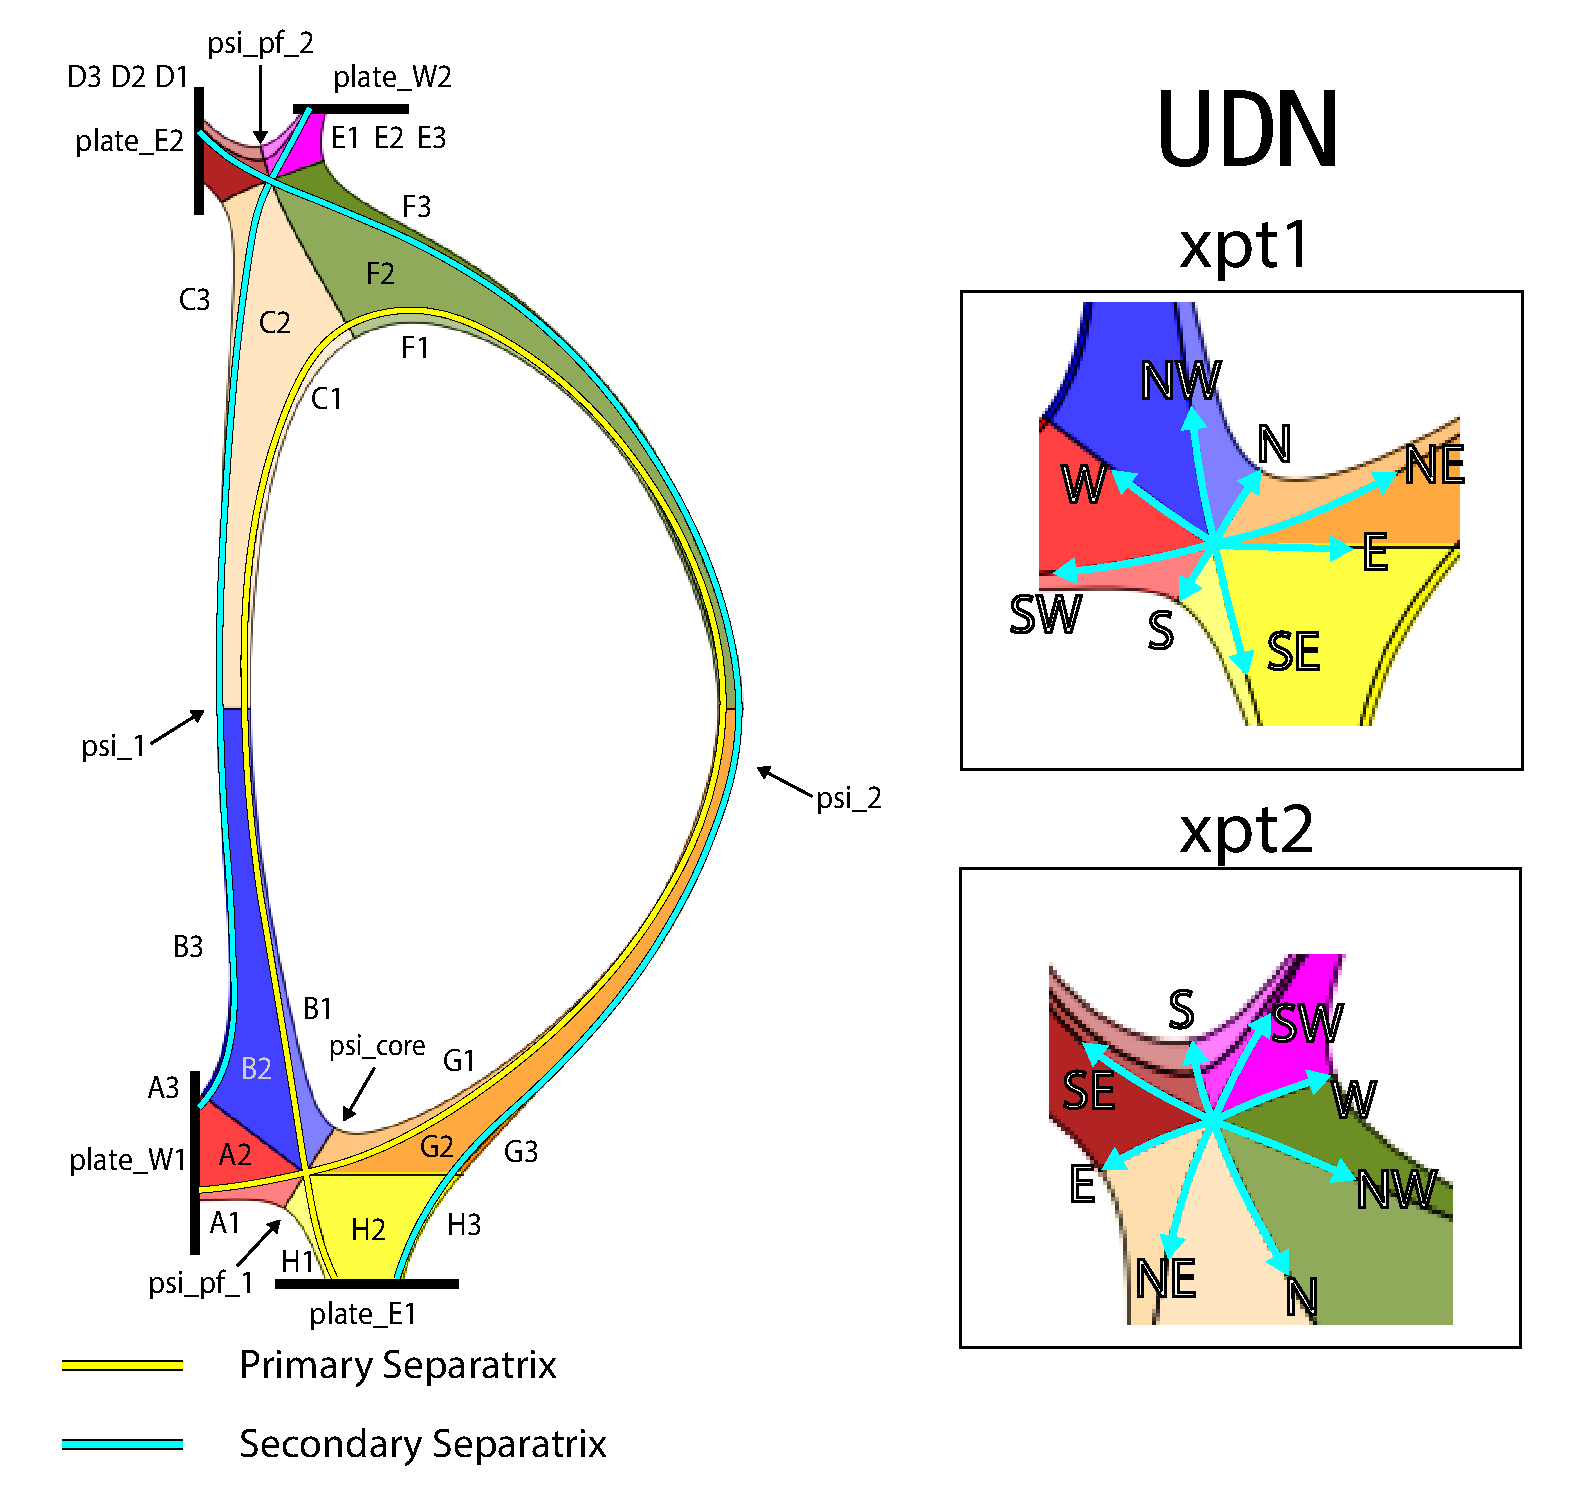
\includegraphics[width=\textwidth]{figures/configurations/UDN_collection.pdf}
        \caption{UDN Patch-Map}
        \label{fig:udn_patch_map}
\end{figure}
\begin{figure}[H]
    \centering
        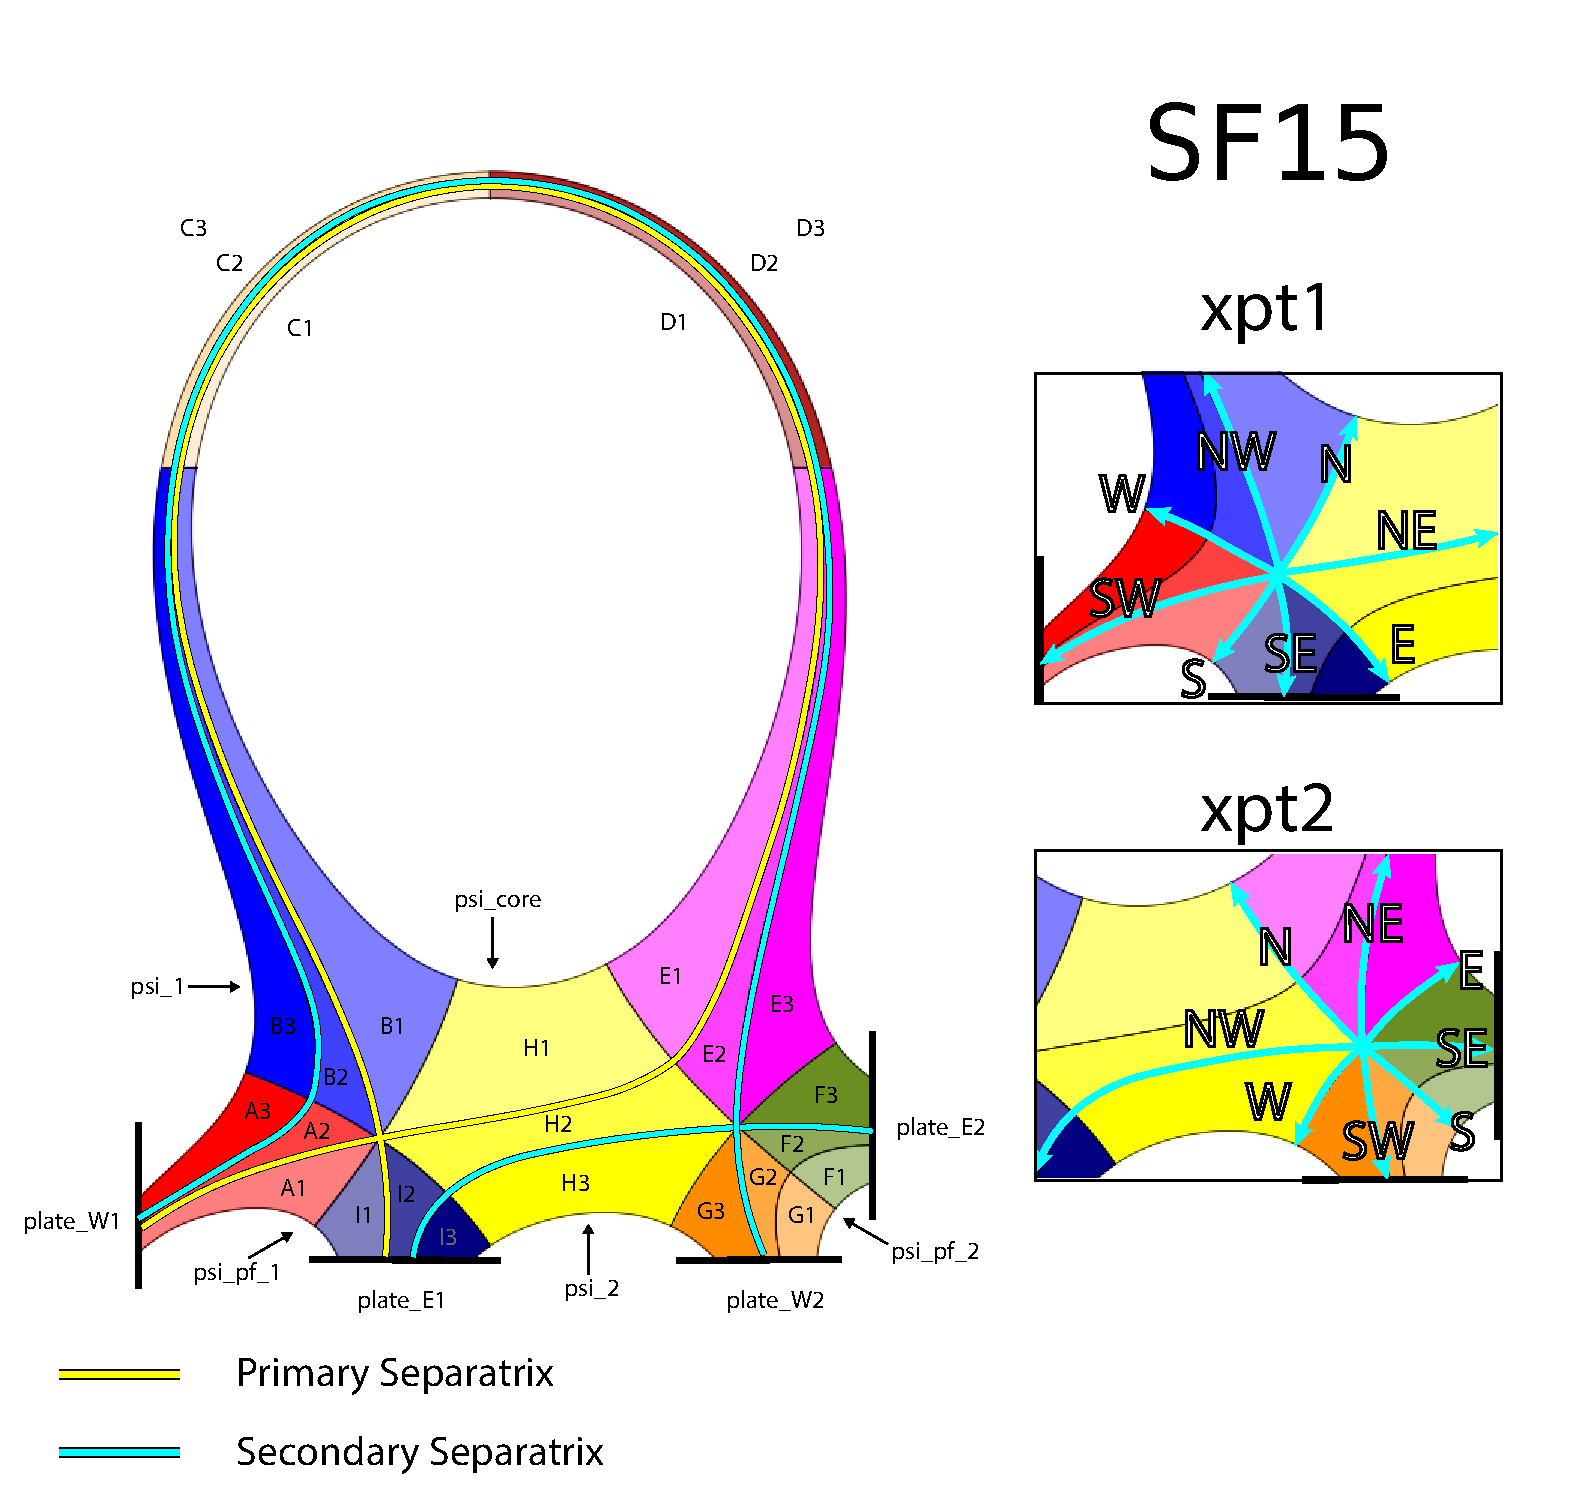
\includegraphics[width=\textwidth]{figures/configurations/SF15_collection.pdf}
        \caption{SF15 Patch-Map}
        \label{fig:sf15_patch_map}
\end{figure}
\begin{figure}[H]
    \centering
        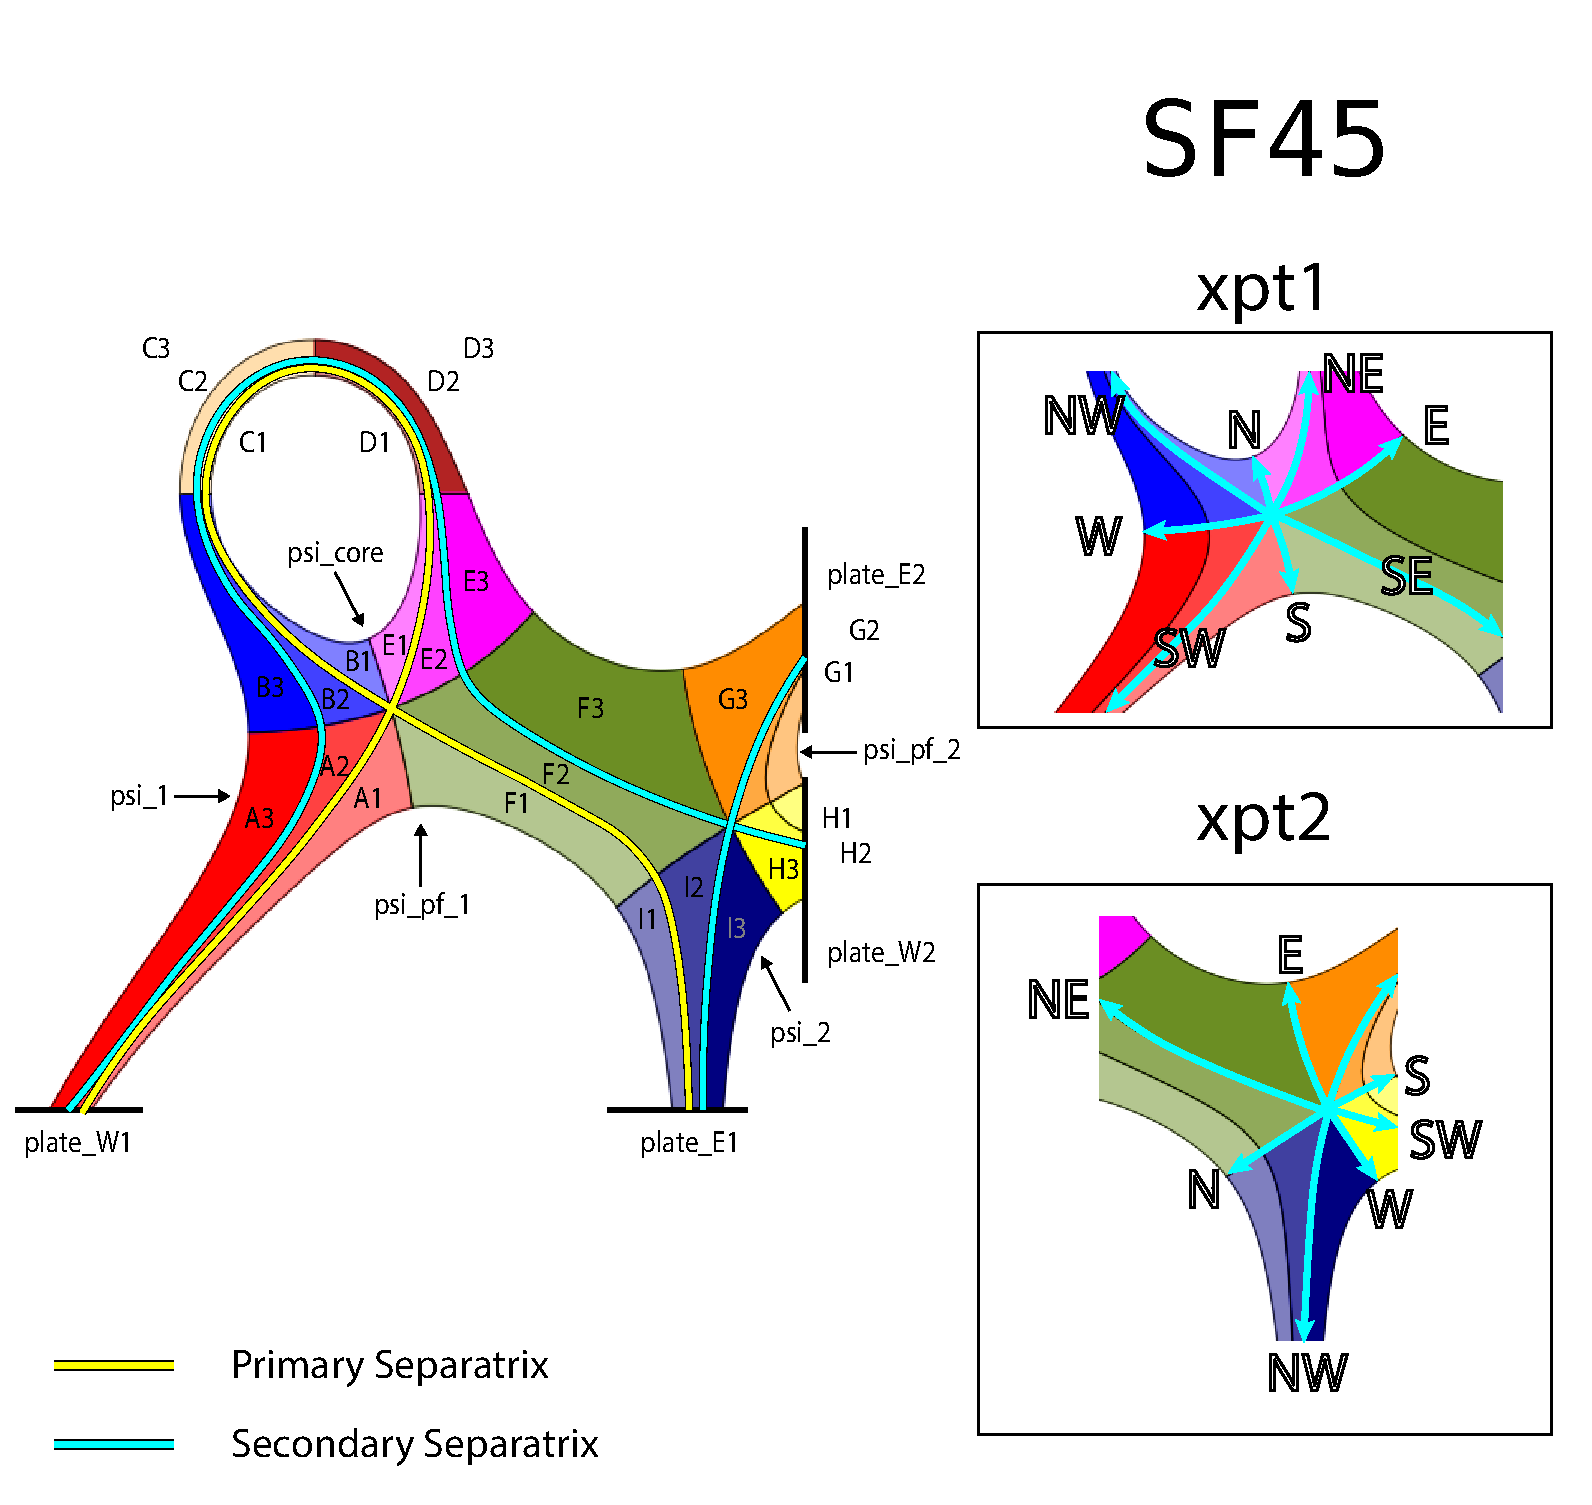
\includegraphics[width=\textwidth]{figures/configurations/SF45_collection.pdf}
        \caption{SF45 Patch-Map}
        \label{fig:sf45_patch_map}
\end{figure}
\begin{figure}[H]
    \centering
        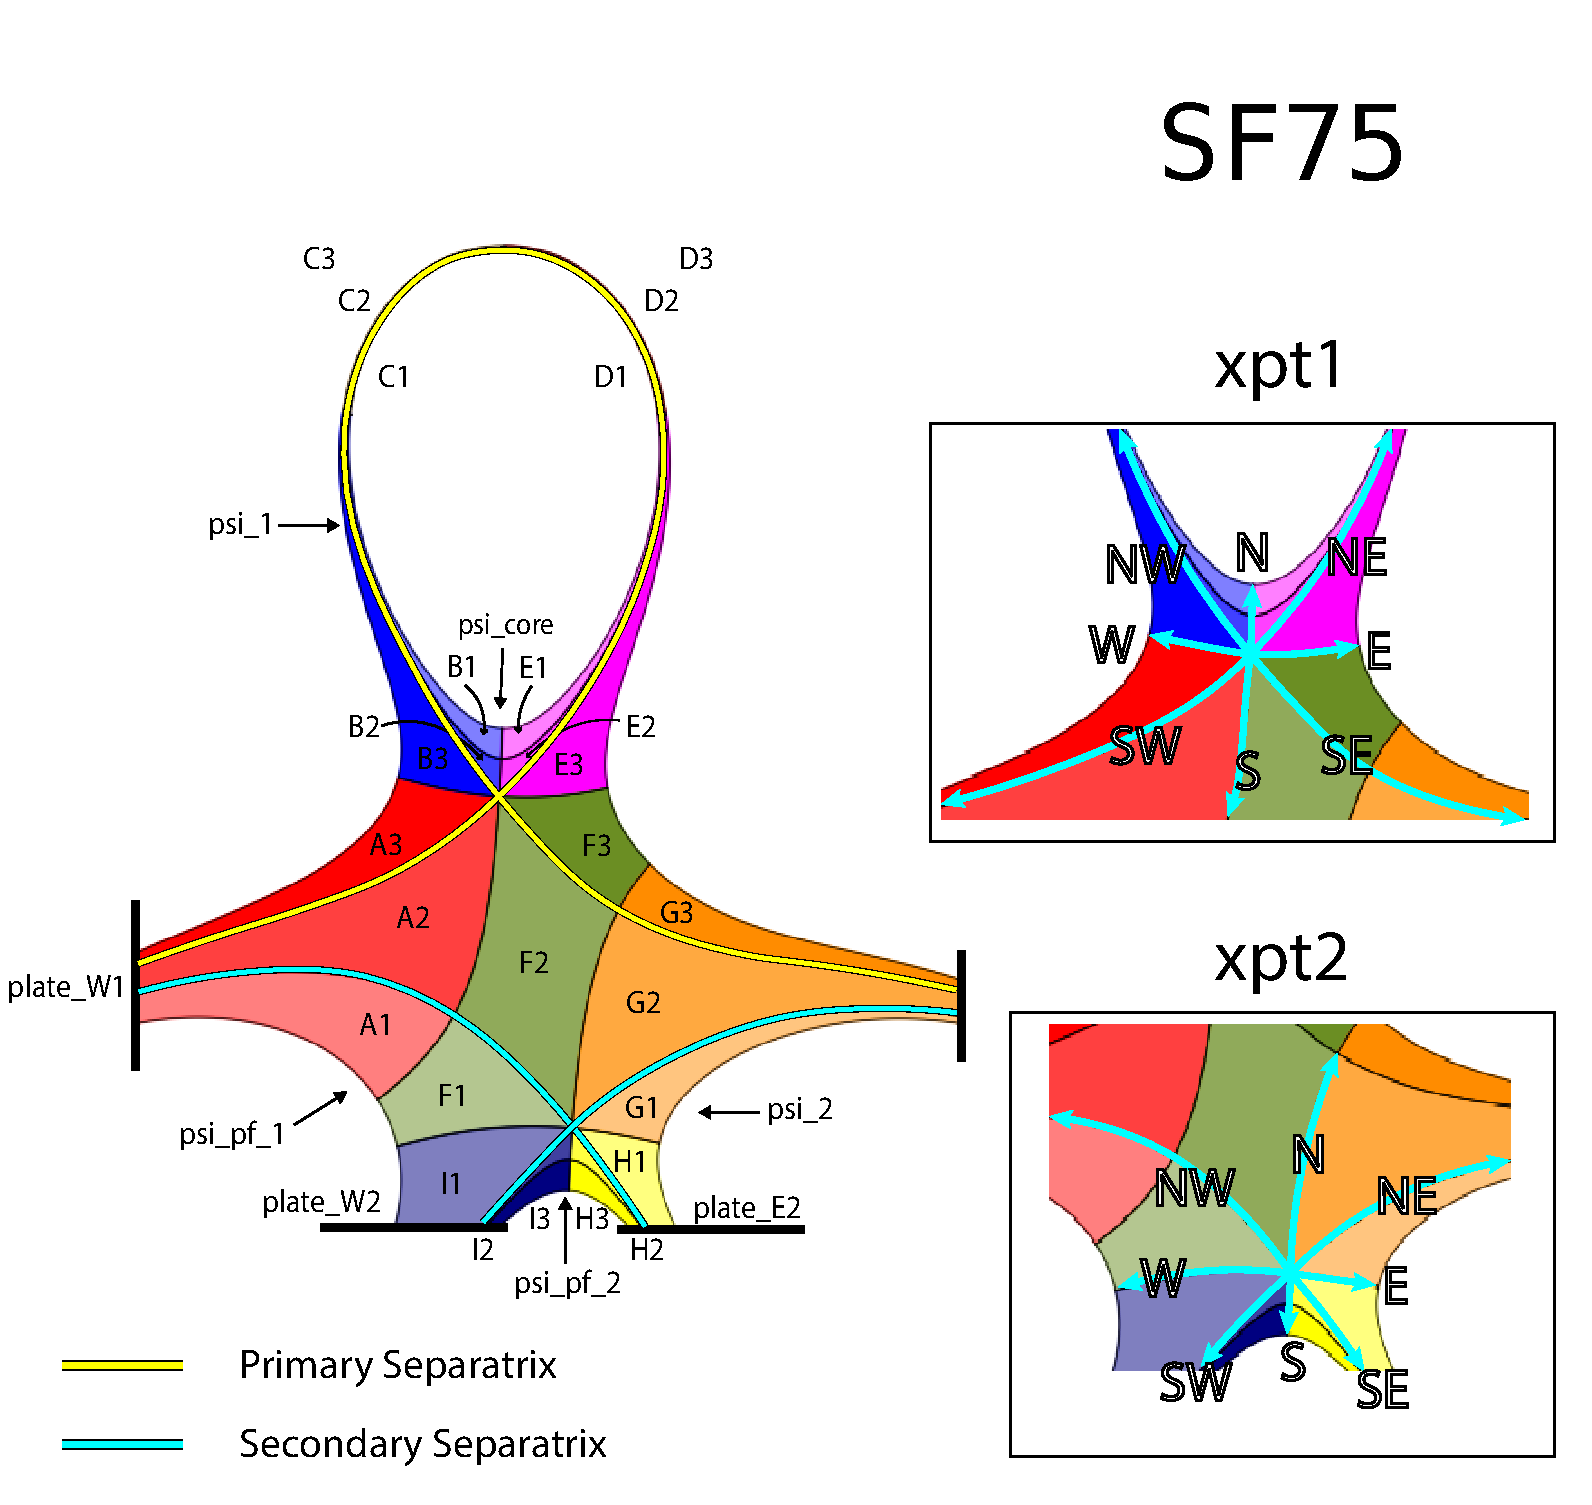
\includegraphics[width=\textwidth]{figures/configurations/SF75_collection.pdf}
        \caption{SF75 Patch-Map}
        \label{fig:sf75_patch_map}
\end{figure}
\begin{figure}[H]
    \centering
        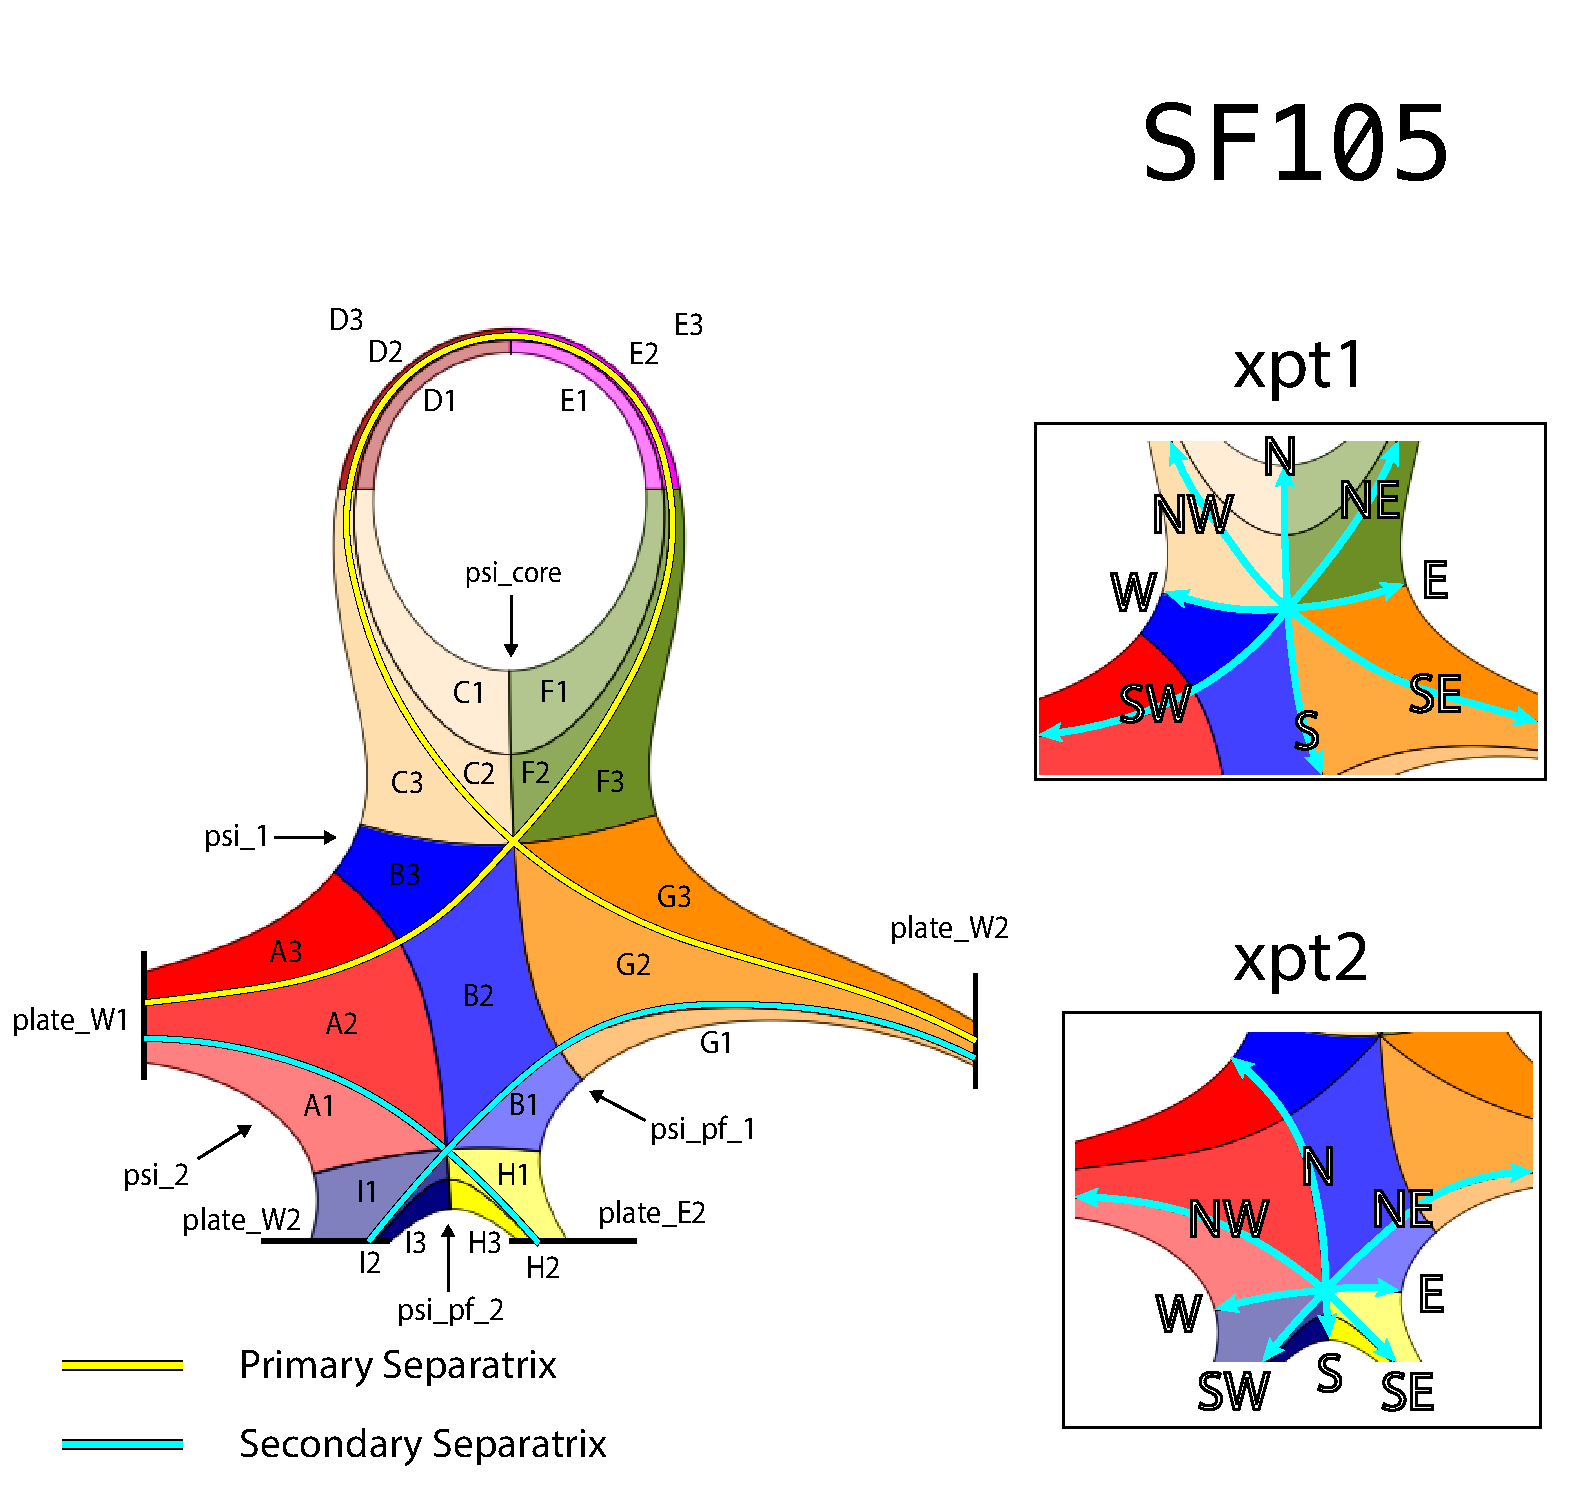
\includegraphics[width=\textwidth]{figures/configurations/SF105_collection.pdf}
        \caption{SF105 Patch-Map}
        \label{fig:sf105_patch_map}
\end{figure}
\begin{figure}[H]
    \centering
        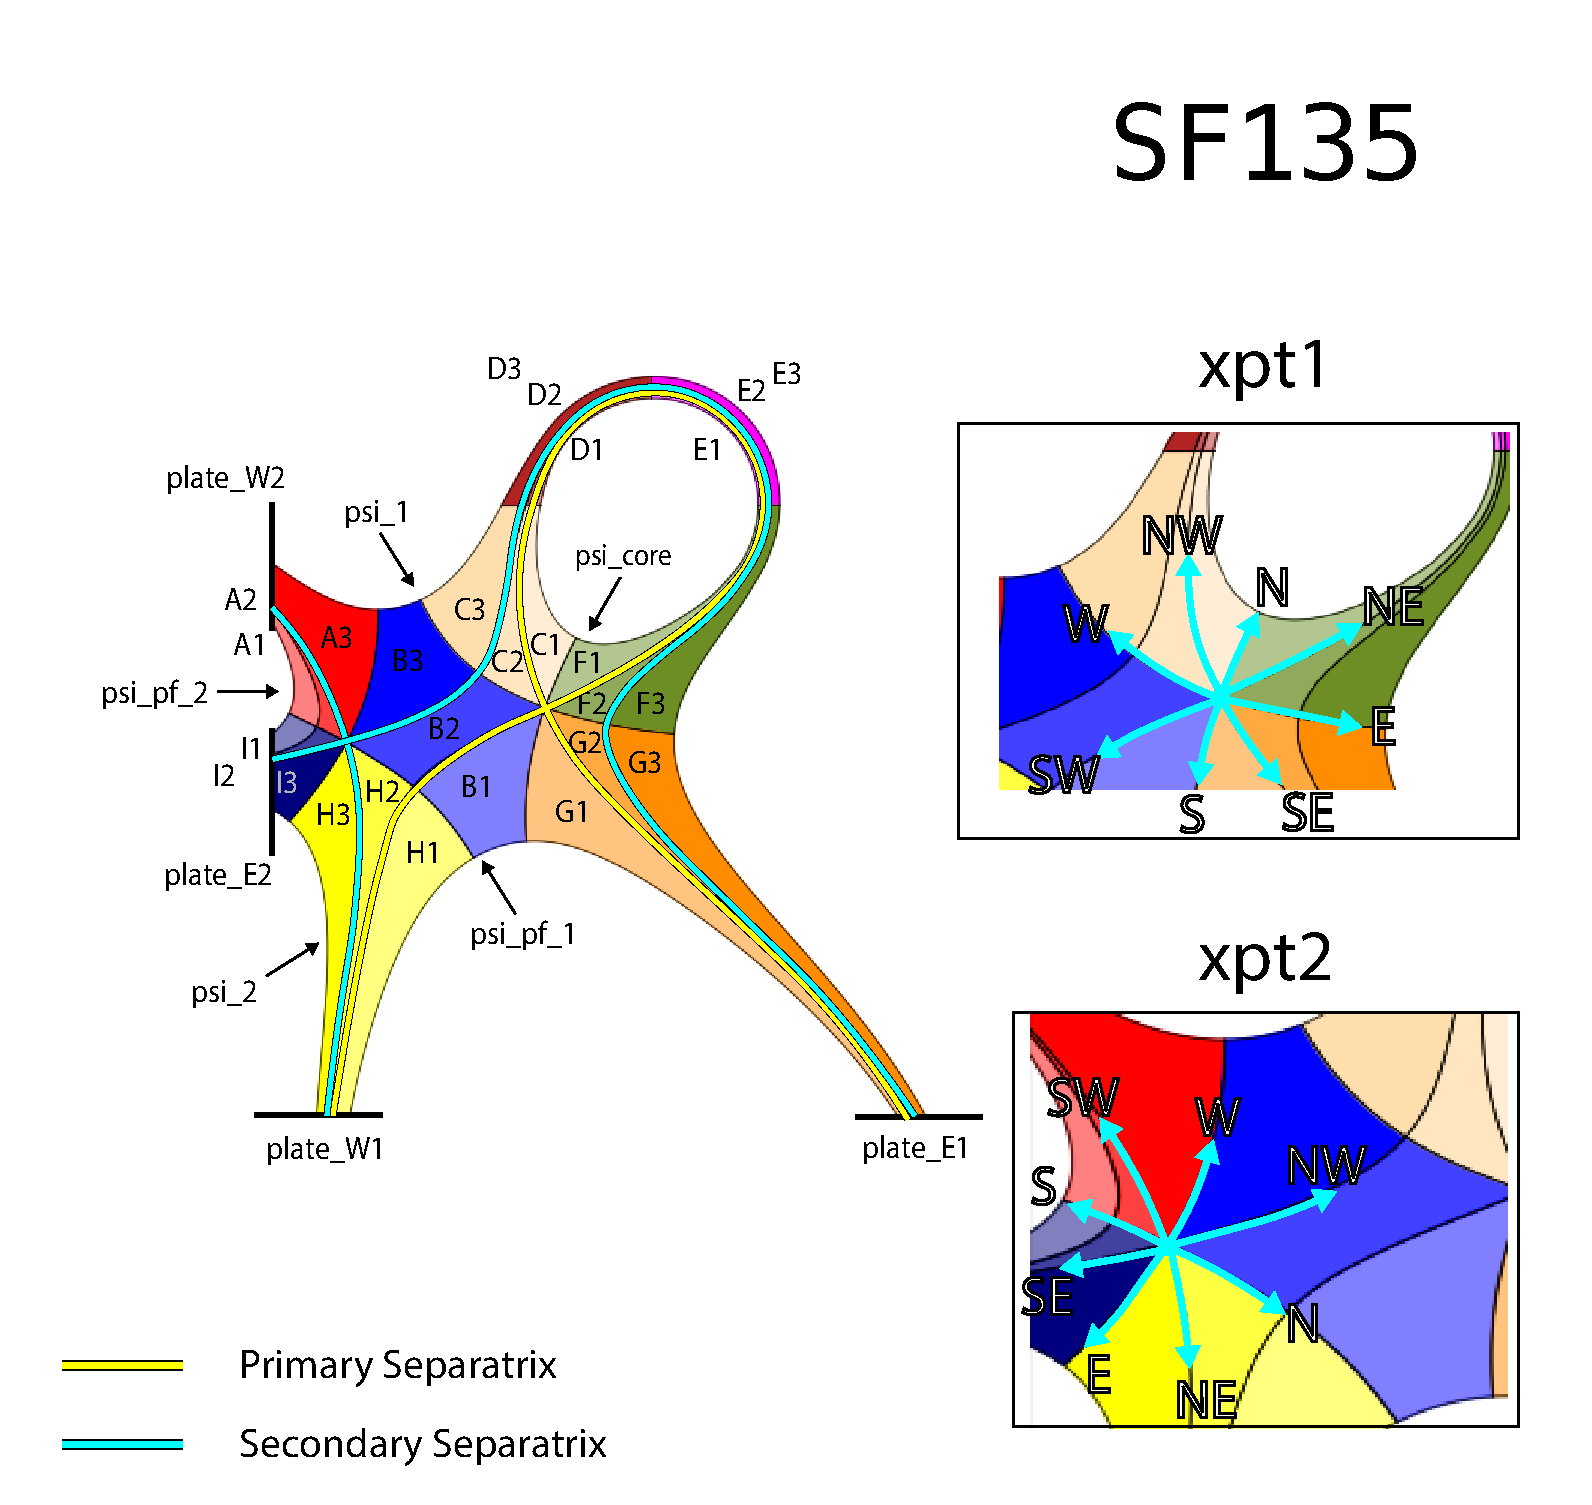
\includegraphics[width=1.05\textwidth]{figures/configurations/SF135_collection.pdf}
        \caption{SF135 Patch-Map}
        \label{fig:sf135_patch_map}
\end{figure}
\begin{figure}[H]
    \centering
        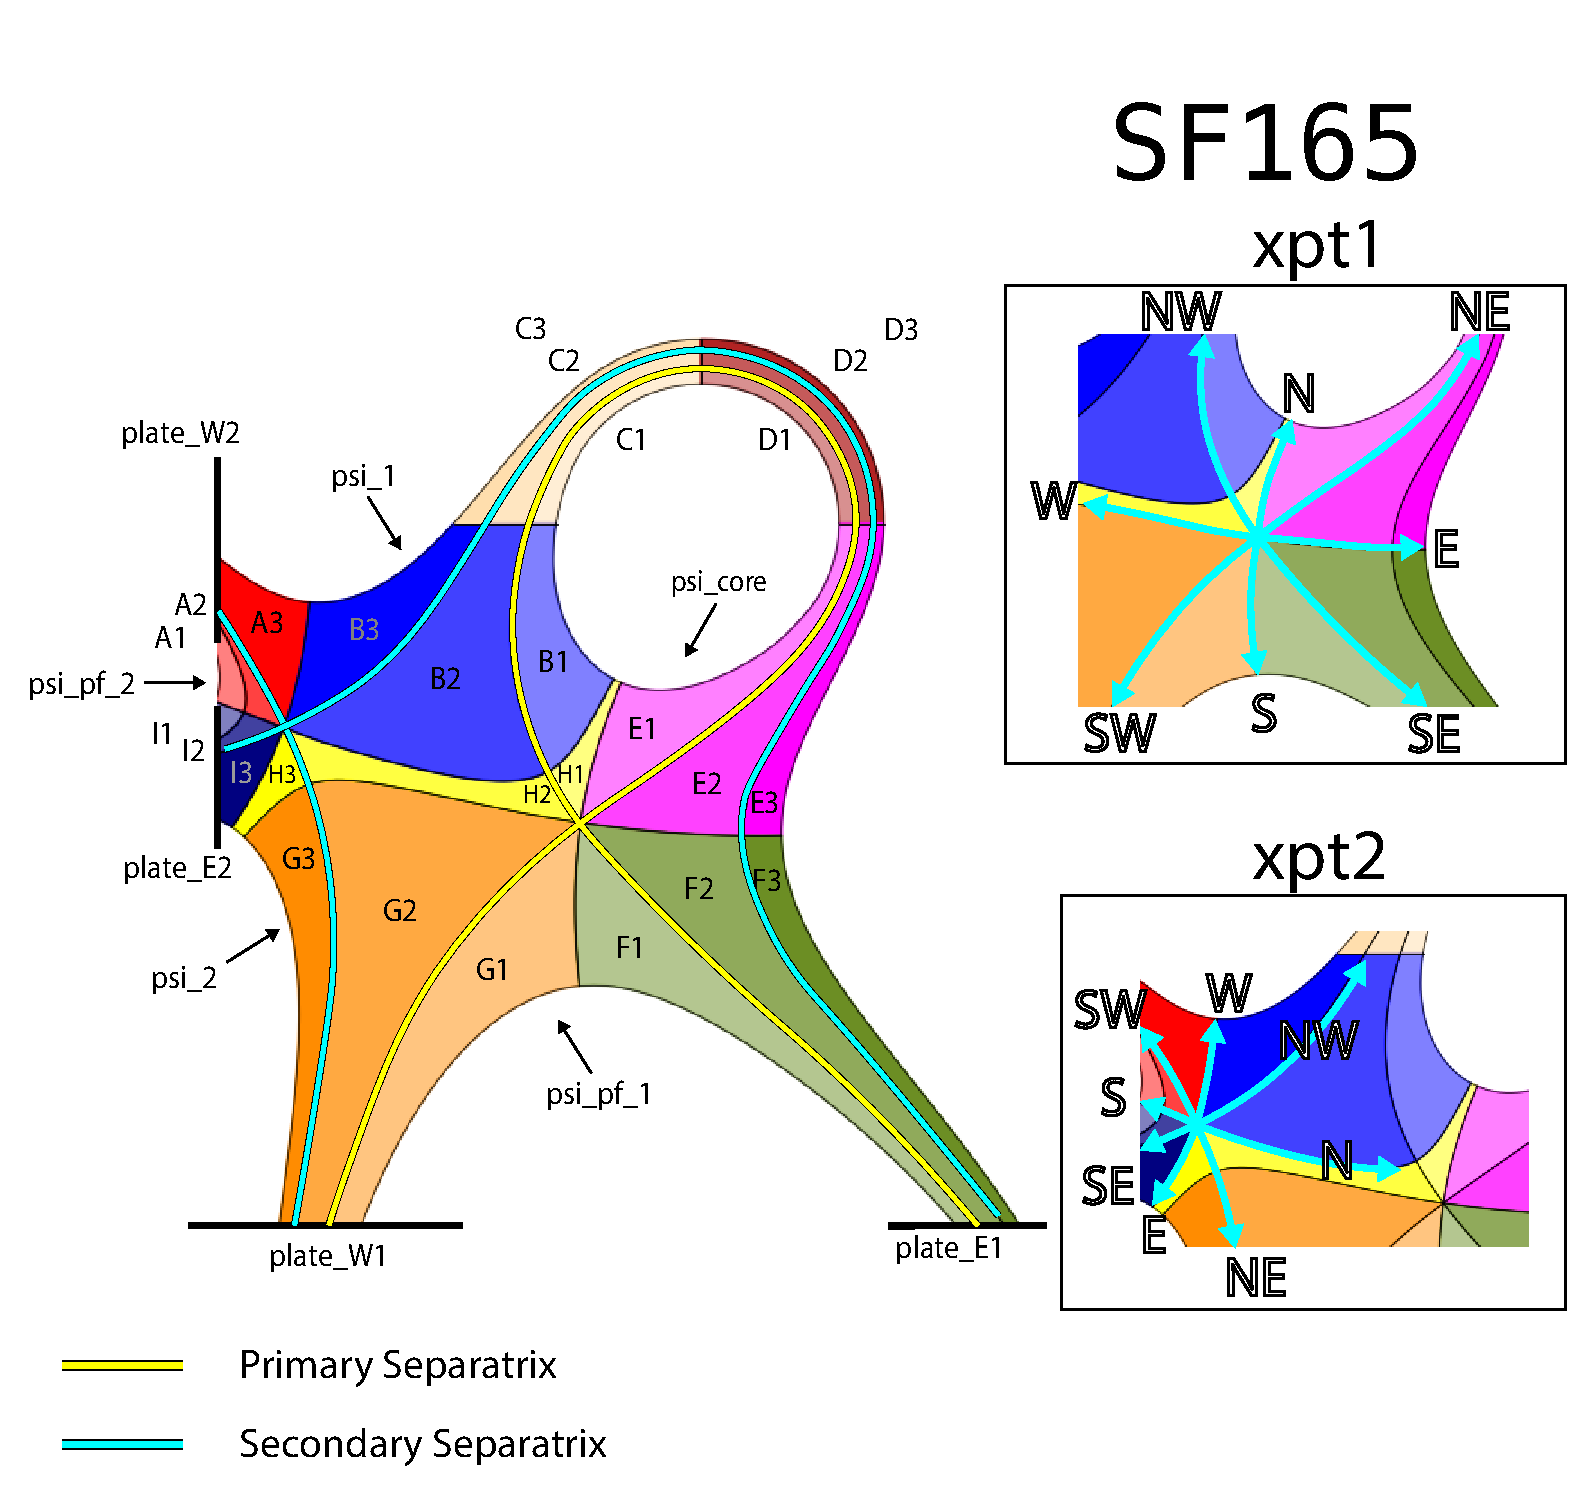
\includegraphics[width=\textwidth]{figures/configurations/SF165_collection.pdf}
        \caption{SF165 Patch-Map}
        \label{fig:sf165_patch_map}
\end{figure}
